\documentclass[a4paper,12pt]{report}

\usepackage[brazil]{babel}
\usepackage[utf8]{inputenc}
\usepackage[T1]{fontenc}
\usepackage[a4paper,margin=2.5cm]{geometry}
\usepackage{graphicx}
\usepackage{longtable}
\usepackage{array}
\usepackage{booktabs}
\usepackage{tabularx}
\usepackage{hyperref}
\usepackage{xcolor}
\usepackage{amssymb}
\usepackage{float}

\title{Quadro digital de avisos}
\author{Grupo 1}
\date{\today}

\begin{document}

\begin{titlepage}
\centering

{\Large Universidade de Brasília -- UnB \par}
{\large Departamento de Ciência da Computação (CIC) \par}
{\large CIC0101 -- Sistemas de Informação \par}

\vspace{2cm}

{\Huge\bfseries Quadro digital de avisos\par}

\vspace{1cm}

{\Large Software Development Plan\par}

\vspace{1cm}

Versão: 1.0

Data: 22/11/2026

\vfill

Grupo: 1

Integrantes:

Calebe Alves Freitas - 222035699

Leonardo Nehrer Sequeira - 221039970

Luan Silveira Alves de Moura - 242012154

Maira Silva de Arruda - 222026214

\end{titlepage}

\tableofcontents

\chapter{Introdução}

\section{Finalidade do documento}
Este Plano de Desenvolvimento de Software tem como finalidade estabelecer a visão, o escopo e as diretrizes técnicas e organizacionais para a concepção de um sistema de informação voltado à centralização e à melhoria da comunicação escolar, inicialmente direcionado a instituições de ensino básico. O sistema proposto busca organizar a troca de informações entre direção, coordenação, secretaria, professores, alunos e responsáveis por meio de um ambiente centralizado para avisos, consulta de informações escolares (como notas, frequências e declarações), acompanhamento de comunicações e canais de contato e atendimento. Este documento permite compreender a integralidade do projeto, reunindo a situação-problema, os objetivos, os limites do escopo, os stakeholders e suas necessidades, os processos e requisitos funcionais, bem como a organização dos dados e regras de negócio que fundamentam a solução.

\section{Problema e justificativa}

\subsection{Problema atual}
A comunicação entre os membros da comunidade escolar ocorre atualmente por diferentes meios, como grupos de WhatsApp, quadros de avisos físicos distribuídos pela escola e comunicados enviados aos responsáveis. Esses canais operam de forma descentralizada e sem padronização do fluxo de comunicação, fazendo com que informações institucionais, pedagógicas e administrativas nem sempre cheguem aos destinatários corretos ou sejam recebidas em tempo hábil.

\subsection{Atores afetados, evidências e consequências observadas}
A descentralização e a falta de um processo estruturado afetam a comunidade escolar em sua totalidade — abrangendo direção, coordenação, secretaria, professores, alunos e responsáveis — e reduzem a eficácia dos avisos, bem como o acompanhamento das atividades escolares por alunos e famílias. Entre as evidências e manifestações observadas estão:

\begin{itemize}
    \item Avisos importantes são perdidos em meio ao grande volume de mensagens dos grupos de WhatsApp.
    \item Nem todos os membros da comunidade escolar participam dos grupos existentes.
    \item Comunicados em quadros de avisos físicos possuem alcance limitado e dependem da presença e da atenção do destinatário na escola.
    \item Responsáveis que trabalham possuem dificuldades para acompanhar as informações escolares.
    \item Há incerteza sobre quem recebeu ou tomou conhecimento de determinados avisos.
    \item O acompanhamento da vida escolar dos alunos ocorre de maneira fragmentada, exigindo consulta a diferentes canais de informação.
\end{itemize}

\subsection{Delimitação do problema}
A escola enfrenta dificuldades para garantir que informações institucionais, pedagógicas e administrativas sejam distribuídas de forma organizada, tempestiva e acessível para todos os membros da comunidade escolar. Mesmo sem considerar uma solução tecnológica específica, a falta de coordenação central, de categorização por tipo e público-alvo, de fluxo formal de publicação/aprovação e de mecanismos de registro de recebimento e leitura mantém o problema existente, comprometendo o acompanhamento das atividades escolares, a participação das famílias e a efetividade da comunicação institucional. Como respostas iniciais a esses sintomas, já foram modeladas medidas como centralizar a divulgação, organizar comunicados por tipo e público-alvo, disponibilizar acompanhamento integrado, estabelecer moderação e validação dos avisos e registrar recebimento e leitura.

\subsection{Justificativa}
A comunicação eficiente é essencial para o funcionamento das atividades escolares e para o fortalecimento da relação entre escola, alunos e responsáveis. Problemas de comunicação podem causar perda de prazos, baixa participação em eventos, dificuldade de acompanhamento do desempenho escolar e redução do engajamento das famílias. Melhorar esse processo contribui para aumentar a transparência institucional, fortalecer a participação da comunidade escolar e apoiar a gestão das atividades educacionais.

\section{Escopo e limites}

\subsection{Incluído no escopo}
\begin{itemize}
    \item Criação de uma plataforma centralizada para comunicação de avisos escolares.
    \item Organização, moderação/autorização, segmentação por público-alvo e divulgação de avisos e comunicados escolares.
    \item Divulgação de notas e frequências, sem afetar os fluxos de trabalho da secretaria.
    \item Controle sobre o envio, recebimento e visualização.
    \item Integração da comunidade escolar (direção, coordenação, secretaria, professores, alunos e responsáveis) em um ambiente centralizado.
    \item Disponibilização de canal de comunicação entre os responsáveis pelos alunos e a escola.
\end{itemize}

\subsection{Fora do escopo}
\begin{itemize}
    \item Não haverá integração com sistemas administrativos e de gestão interna da escola, tais como controle financeiro, gestão de funcionários e fluxos de trabalho da secretaria.
    \item Não haverá substituição dos processos pedagógicos existentes.
\end{itemize}

\chapter{Visão geral do projeto}

\section{Objetivos e resultados esperados}

\subsection{Objetivo geral}
Desenvolver um sistema de informação que centralize e facilite a comunicação entre a comunidade escolar, promovendo maior eficiência na troca de informações entre a direção, professores da instituição e os responsáveis e alunos, por meio da disponibilização de avisos, notas, frequências, declarações e canais de contato.

\subsection{Objetivos específicos}
\begin{enumerate}
    \item Reduzir a perda e a dispersão de informações na comunicação entre a escola, os responsáveis e os alunos.
    \item Disponibilizar uma plataforma centralizada e de fácil acesso para consulta de informações escolares e de desempenho dos alunos.
    \item Promover um canal de comunicação para o envio de feedbacks, dúvidas e solicitações por parte dos responsáveis e alunos.
\end{enumerate}

Os objetivos buscam solucionar as principais dificuldades de comunicação e acesso às informações existentes no ambiente escolar, tornando a comunicação entre direção, professores, alunos e responsáveis mais organizada, ágil e eficiente.

\subsection{Resultados e benefícios esperados}

\textbf{Para os usuários:}
\begin{itemize}
    \item Acesso mais organizado, tempestivo e centralizado a avisos, atividades, eventos e informações acadêmicas (notas e frequências), reduzindo a fragmentação entre múltiplos canais.
    \item Maior facilidade no acompanhamento da vida escolar dos alunos, inclusive para responsáveis com rotina de trabalho, favorecendo o engajamento das famílias e a redução da perda de prazos ou baixa participação em eventos.
    \item Canal estruturado e documentado para responsáveis e tutores legais enviarem dúvidas, feedbacks e solicitações e receberem retornos de forma mais ágil e clara.
\end{itemize}

\textbf{Para a escola:}
\begin{itemize}
    \item Maior organização e controle no fluxo de divulgação e moderação/validação dos comunicados institucionais, reduzindo ruídos e perdas de informação.
    \item Aumento da transparência institucional, fortalecimento da participação da comunidade escolar e apoio à gestão das atividades educacionais.
    \item Maior agilidade no direcionamento e no tempo de resposta às solicitações encaminhadas à área administrativa/responsáveis competentes.
\end{itemize}

\section{Stakeholders e necessidades}

A Tabela~\ref{tab:stakeholders} apresenta os stakeholders identificados no contexto de comunicação escolar, destacando o papel de cada um no cenário atual (AS-IS) e suas respectivas necessidades de informação.

\begin{longtable}{|p{3.2cm}|p{5.2cm}|p{6.2cm}|}
\caption{Papéis no processo atual (AS-IS) e necessidades de informação.} \label{tab:stakeholders} \\
\hline
\textbf{Stakeholder} & \textbf{Papel no processo} & \textbf{Necessidade de informação} \\
\hline
\endfirsthead
\hline
\textbf{Stakeholder} & \textbf{Papel no processo} & \textbf{Necessidade de informação} \\
\hline
\endhead
\textbf{Emissor do aviso} \newline \textit{(direção, coordenação, professor)} & Produz e divulga avisos e comunicados escolares por canais como quadros de avisos físicos, comunicados impressos/enviados em padronização, bilhetes, grupos de WhatsApp sem controle. & Necessidade de divulgar comunicados de forma estruturada e alcançar os destinatários corretos com segurança sobre o conteúdo e sua validação, evitando perdas no volume de mensagens ou alcance restrito ao ambiente físico. \textit{Ex.: comunicar suspensão de aulas em três salas apenas aos envolvidos.} \\
\hline
\textbf{Avaliador} \newline \textit{(direção, coordenação, secretaria)} & Acompanha e organiza a divulgação de comunicados e o encaminhamento de informações na rotina escolar, enfrentando falta de fluxo formal e centralizado. & Necessidade de filtrar, validar e direcionar adequadamente o que é comunicado na escola, reduzindo ruídos, bloqueando informações inadequadas ou inviáveis e tendo controle sobre a divulgação. \textit{Ex.: verificar se um comunicado atende às condições necessárias antes de circular.} \\
\hline
\textbf{Destinatários} \newline \textit{(tutor, comunidade escolar)} & Recebem comunicados e buscam acompanhar informações escolares por diferentes canais (WhatsApp, murais, quadros de avisos, bilhetes). & Necessidade de acessar informações relevantes no tempo adequado e de forma organizada, sem perder avisos importantes em meio a excesso de mensagens ou depender de presença física na escola. \textit{Ex.: receber comunicados do próprio interesse sem sobrecarga de avisos dispersos.} \\
\hline
\textbf{Tutor do aluno} & Acompanha a vida escolar do aluno e busca comunicar-se com a escola sobre questões particulares ou rotineiras. & Necessidade de contar com um canal claro e documentado para tratar de demandas particulares com a escola e obter retorno, evitando informações fragmentadas, ligações informais ou deslocamentos presenciais. \textit{Ex.: informar ausência do aluno por motivo familiar por meio registrado.} \\
\hline
\textbf{Respondente} \newline \textit{(direção, coordenação, professor)} & Lida com dúvidas, solicitações e demandas vindas da comunidade escolar no dia a dia, muitas vezes por canais dispersos. & Necessidade de identificar com clareza as demandas de sua competência, evitar encaminhamentos desordenados e dar retorno organizado e tempestivo aos solicitantes. \textit{Ex.: analisar uma solicitação recebida referente à sua atuação e emitir resposta adequada.} \\
\hline
\end{longtable}

\section{Premissas, restrições e riscos}

\subsection{Premissas e hipóteses}
As seguintes premissas e hipóteses orientam a concepção inicial do projeto, devendo ser confirmadas junto ao contexto real da instituição escolar:
\begin{itemize}
    \item Assume-se como público-alvo da aplicação instituições de ensino básico, com foco na comunicação entre direção, coordenação, secretaria, professores, alunos e responsáveis.
    \item Parte-se da premissa de que o sistema apoiará a interação, divulgação de informações, consulta de indicadores acadêmicos e troca de mensagens, sem substituir os processos pedagógicos e administrativos existentes na escola.
    \item Assume-se, como hipótese de trabalho a ser verificada na organização, que as perdas, atrasos e incertezas de recebimento decorrem da dispersão entre múltiplos canais sem coordenação central, da falta de categorização por tipo e público-alvo, da ausência de fluxo formal de publicação/aprovação e da falta de acompanhamento de recebimento e leitura.
    \item Considera-se como hipótese de modelagem que a obrigatoriedade de moderação prévia depende de diretrizes ou categorias definidas pela escola, ainda sujeitas a confirmação formal.
\end{itemize}

\subsection{Restrições e limitações}
\begin{itemize}
    \item O projeto não abrange sistemas administrativos e de gestão interna da escola (como controle financeiro, gestão de funcionários e fluxos de trabalho da secretaria).
    \item As categorias de avisos que exigem aprovação prévia dependem de processos decisórios da direção ou conselho escolar. Diante da flexibilidade de regras institucionais, a modelagem inicial considera a possibilidade de moderação prévia para todos os avisos, com posterior refinamento das regras de negócio.
    \item Como premissa de controle de acesso a ser validada com a instituição, o acesso aos dados e às ações do sistema segue a lógica por perfil: direção e coordenação acessam todos os dados; a secretaria acessa notas e frequência de todos os alunos; professores acessam somente dados de suas turmas; alunos acessam apenas os seus próprios dados; responsáveis e tutores legais acessam dados de seus tutelados; apenas funcionários da escola podem postar avisos; e somente direção, coordenação e secretaria podem aprovar avisos.
    \item A operação do sistema depende do alinhamento ao calendário escolar, da tempestividade e da relevância dos avisos para evitar excesso de mensagens e garantir entrega oportuna aos destinatários, priorizando recursos voltados a dispositivos móveis para assegurar notificações eficientes e acesso ágil a comunidade escolar.
\end{itemize}

\subsection{Riscos identificados}
\begin{itemize}
    \item A ausência de definição prévia sobre categorias que exigem moderação, fluxos de aprovação e regras acadêmicas ou de vínculo pode exigir ajustes posteriores no modelo de dados e nas regras do sistema.
    \item A publicação de avisos sem critério de relevância, tempestividade ou segmentação adequada por público-alvo pode gerar ruído, sobrecarga de notificações ou não alcançar os destinatários corretos.
    \item Problemas de conectividade, indisponibilidade de canais de notificação ou ausência de confirmação de leitura podem comprometer o recebimento oportuno e a ciência dos comunicados.
    \item Falhas na aplicação da segregação de acesso por perfil (direção, coordenação, secretaria, professores, alunos e responsáveis/tutores) podem expor informações restritas ou permitir ações indevidas de publicação e aprovação.
    \item O não alinhamento ao calendário escolar ou dificuldades de desempenho e notificação em dispositivos móveis podem reduzir o engajamento da comunidade escolar e a efetividade do quadro de avisos.
\end{itemize}

\chapter{Sistema de Informação e contexto organizacional}

\section{Visão sistêmica}

O sistema proposto atua como um hub centralizado de comunicação e acompanhamento escolar, organizando o fluxo de informações entre os diferentes perfis da instituição. Seus componentes estruturais são definidos da seguinte forma:

\begin{itemize}
    \item \textbf{Limites do sistema:} a fronteira da aplicação abrange a criação, moderação, segmentação e divulgação de avisos escolares, a consulta de informações acadêmicas (notas, frequências e declarações) e o canal de troca de mensagens e atendimento entre responsáveis/alunos e a escola. Ficam fora da fronteira do sistema os processos internos de gestão administrativa, financeira, recursos humanos, matrículas e rotinas operacionais da secretaria, bem como a substituição das atividades pedagógicas existentes.
    
    \item \textbf{Entradas:} o sistema recebe dados cadastrais e de vínculo institucional (perfis de direção, coordenação, secretaria, professores, alunos e responsáveis/tutores), conteúdos de avisos e comunicados elaborados pelos funcionários autorizados (acompanhados de categoria, nível de urgência e público-alvo), decisões de aprovação ou indeferimento emitidas pelos avaliadores, registros acadêmicos disponibilizados para consulta (notas e frequências) e solicitações, dúvidas ou feedbacks enviados por responsáveis e alunos.
    
    \item \textbf{Processamento:} as entradas são tratadas por meio de regras de negócio e controle de acesso por perfil. O sistema valida permissões de atuação e visibilidade, submete os comunicados ao fluxo de moderação/autorização (quando aplicável), segmenta e direciona os avisos conforme o público-alvo e o calendário escolar, encaminha solicitações ao respondente competente e registra os eventos de envio, recebimento e visualização das mensagens.
    
    \item \textbf{Saídas:} como resultado do processamento, o sistema entrega notificações direcionadas (prioritariamente em dispositivos móveis), exibe o mural centralizado de avisos segmentados por perfil, disponibiliza consultas estruturadas de notas e frequências, apresenta respostas oficiais às solicitações encaminhadas e gera registros de acompanhamento sobre entrega e leitura dos comunicados.
    
    \item \textbf{Ambiente:} o sistema opera no contexto organizacional de instituições de ensino básico, interagindo diretamente com a comunidade escolar (direção, coordenação, secretaria, professores, alunos e responsáveis) e condicionando sua operação ao calendário acadêmico, às diretrizes internas de comunicação da escola e à infraestrutura de conectividade e dispositivos móveis dos usuários.
    
    \item \textbf{Interfaces:} a interação principal ocorre por meio de interfaces gráficas voltadas prioritariamente para dispositivos móveis (com suporte a acesso web), adaptadas às permissões de cada perfil de usuário. Adicionalmente, o sistema utiliza serviços de notificação push para alertar os destinatários sobre novos avisos e retornos de atendimento.
    
    \item \textbf{Mecanismos de feedback:} a retroalimentação do sistema ocorre em três níveis: (i) \textit{acompanhamento de comunicação}, por meio do registro de envio, entrega e confirmação de leitura/ciência dos avisos pelos destinatários; (ii) \textit{retorno de atendimento}, mediante o fluxo de envio de dúvidas, justificativas ou solicitações pelos responsáveis/alunos e o registro das respostas oficiais da escola; e (iii) \textit{controle de moderação}, pelo retorno motivado de aprovação ou indeferimento dado aos emissores de avisos antes da publicação.
\end{itemize}

\section{Pessoas, processos, dados e tecnologia}

Um sistema de informação funciona como um sistema sociotécnico no qual o valor surge com o alinhamento entre o subsistema social — composto por pessoas, processos, papéis e tomada de decisão — e o subsistema técnico (formado por tecnologia e dados). A Tabela~\ref{tab:ppdt} sintetiza como esses quatro componentes se articulam no sistema proposto, relacionando a aplicação prática de cada um às evidências e aos artefatos do projeto.

\begin{longtable}{|p{2.5cm}|p{6.8cm}|p{5.3cm}|}
\caption{Articulação entre pessoas, processos, dados e tecnologia no projeto.} \label{tab:ppdt} \\
\hline
\textbf{Componente} & \textbf{Aplicação concreta no projeto} & \textbf{Evidência/artefato} \\
\hline
\endfirsthead
\hline
\textbf{Componente} & \textbf{Aplicação concreta no projeto} & \textbf{Evidência/artefato} \\
\hline
\endhead
\textbf{Pessoas} & Direção, coordenação, secretaria, professores, alunos e responsáveis/tutores legais atuam com papéis, responsabilidades e permissões segregadas — apenas funcionários postam avisos; somente direção, coordenação e secretaria aprovam comunicados; direção e coordenação acessam todos os dados; secretaria consulta notas e frequências de todos; professores acessam apenas suas turmas; alunos acessam os próprios dados; e responsáveis/tutores acessam os dados de seus tutelados —, além de tomarem decisões e poderem aderir, adaptar ou contornar fluxos caso o sistema não atenda à rotina real. & Mapeamento de stakeholders e necessidades (Tabela~\ref{tab:stakeholders}), regras de controle de acesso por perfil e cadastro institucional de usuários e vínculos. \\
\hline
\textbf{Processos} & Estruturação dos fluxos de criação, moderação/autorização, segmentação por público-alvo e publicação de avisos; acompanhamento de envio, recebimento e leitura; consulta de notas, frequências e declarações; e troca de mensagens para dúvidas, justificativas e solicitações com retorno oficial, operando alinhados ao calendário escolar sem substituir rotinas internas e evitando desalinhamentos entre o fluxo real e a ferramenta. & Delimitação de escopo e limites, requisitos funcionais, fluxos operacionais do sistema (elaboração, validação, divulgação, leitura e atendimento) e calendário acadêmico. \\
\hline
\textbf{Dados} & Servem de base coletada por pessoas e processos, processada pela tecnologia e interpretada para gerar informação de acompanhamento e apoio à decisão: cadastros de usuários e vínculos (perfis, turmas, alunos e tutelados), conteúdos e metadados dos avisos (categoria, urgência, relevância e destinatários), pareceres de moderação, registros de entrega e leitura, indicadores acadêmicos consultados e histórico de mensagens/respostas. & Modelo Entidade-Relacionamento (MER), regras de negócio e registros de moderação, leitura e atendimento. \\
\hline
\textbf{Tecnologia} & Viabiliza coleta, processamento, armazenamento e comunicação por meio de aplicação com prioridade para dispositivos móveis, banco de dados, serviços e notificações \textit{push}, aplicando controle de acesso por perfil, roteamento segmentado e rastreamento de leitura e atendimento, mantida apartada de sistemas internos de gestão administrativa, financeira ou de matrículas. & Requisitos operacionais e técnicos (acesso \textit{mobile-first}, serviço de notificações, segregação de perfis) e arquitetura da aplicação. \\
\hline
\end{longtable}

\section{Dados, informação, conhecimento e decisão}

No sistema proposto, registros brutos só geram valor quando contextualizados e organizados para se tornarem informação compreensível, quando articulados à experiência e à interpretação dos atores para formar conhecimento e quando preservados quanto à qualidade (precisão, completude, atualidade, consistência, relevância e acessibilidade), à segurança (confidencialidade, integridade e disponibilidade), à finalidade e à minimização de dados. A coleta restringe-se ao necessário para cada finalidade, respeitando as permissões por perfil e o papel complementar da plataforma em relação às rotinas internas da escola.

A transição entre os níveis ocorre quando, por exemplo, um registro numérico isolado ou um estado de leitura ganha contexto de turma, disciplina, aviso ou prazo para orientar ações. O Quadro~\ref{tab:dicd} apresenta exemplos concretos aplicados ao projeto, identificando os níveis organizacionais envolvidos e o tipo de apoio oferecido.

\begin{longtable}{|p{3.0cm}|p{3.3cm}|p{3.4cm}|p{4.9cm}|}
\caption{Exemplos de dados, informações, conhecimento, apoio à decisão e níveis organizacionais no projeto.} \label{tab:dicd} \\
\hline
\textbf{Dados coletados} & \textbf{Informações produzidas} & \textbf{Conhecimento e decisões apoiadas} & \textbf{Nível organizacional e tipo de apoio} \\
\hline
\endfirsthead
\hline
\textbf{Dados coletados} & \textbf{Informações produzidas} & \textbf{Conhecimento e decisões apoiadas} & \textbf{Nível organizacional e tipo de apoio} \\
\hline
\endhead
Texto do aviso, categoria, urgência/relevância, turma/público-alvo, data/hora de criação e parecer de aprovação ou indeferimento. & Mural segmentado com avisos validados por turma/perfil, status de moderação e histórico de comunicados ativos e expirados no calendário escolar. & Compreensão sobre gargalos de aprovação ou sobrecarga de comunicados; decisão de aprovar, ajustar ou indeferir avisos, reprogramar envios conforme o calendário e refinar critérios de segmentação. & \textbf{Operacional e tático:} apoio à execução diária e ao controle/coordenação do fluxo de comunicação. \\
\hline
Registros de entrega de notificação, data/hora de visualização e confirmação de leitura por usuário/responsável. & Taxa e listagem de leitura ou não leitura de um comunicado específico por turma ou responsável dentro do prazo. & Identificação de padrões de ciência ou ausência de retorno em avisos críticos; decisão de reenviar lembrete direcionado, acionar responsáveis por outro meio quando necessário ou ajustar horários de notificação. & \textbf{Operacional e tático:} monitoramento de rotinas e acompanhamento gerencial de alcance e engajamento. \\
\hline
Notas, frequências e declarações disponibilizadas para consulta, vinculadas a aluno, turma, período e perfil autorizador. & Boletim de consulta de notas e frequências do próprio aluno ou tutelado (e visão por turma ao professor ou geral conforme permissão). & Percepção precoce de queda de desempenho ou faltas recorrentes; decisão do responsável de dialogar com a escola ou acompanhar o estudante, e do professor/coordenação de revisar estratégias pedagógicas ou de acompanhamento. & \textbf{Operacional e tático:} apoio ao acompanhamento cotidiano e à coordenação pedagógica. \\
\hline
Mensagens de dúvidas, justificativas de ausência ou solicitações enviadas por responsáveis/alunos, perfil de origem, assunto e respostas registradas. & Fila estruturada de mensagens por competência, tempo de resposta e histórico documentado de atendimentos e retornos. & Reconhecimento de temas recorrentes de dúvidas ou justificativas na comunidade escolar; decisão de responder demandas pontuais, redistribuir encaminhamentos ou publicar avisos preventivos para reduzir dúvidas repetitivas. & \textbf{Operacional, tático e estratégico:} apoio ao atendimento cotidiano, à gestão do tempo de resposta e ao aprimoramento de políticas de comunicação institucional. \\
\hline
\end{longtable}

A utilidade dessas informações varia conforme o papel e o momento de quem as acessa, exigindo coerência entre os registros e controle rigoroso de acesso para que decisões não sejam tomadas sobre dados incompletos, desatualizados, inconsistentes ou expostos indevidamente.

\chapter{Análise dos processos}

\section{Processo atual — BPMN AS-IS}

O processo atual de comunicação escolar foi modelado em BPMN (Figura~\ref{fig:bpmn-asis}) para retratar como a divulgação de avisos ocorre na ausência de uma plataforma centralizada e de mecanismos nativos de confirmação de entrega.

\begin{figure}[H]
    \centering
    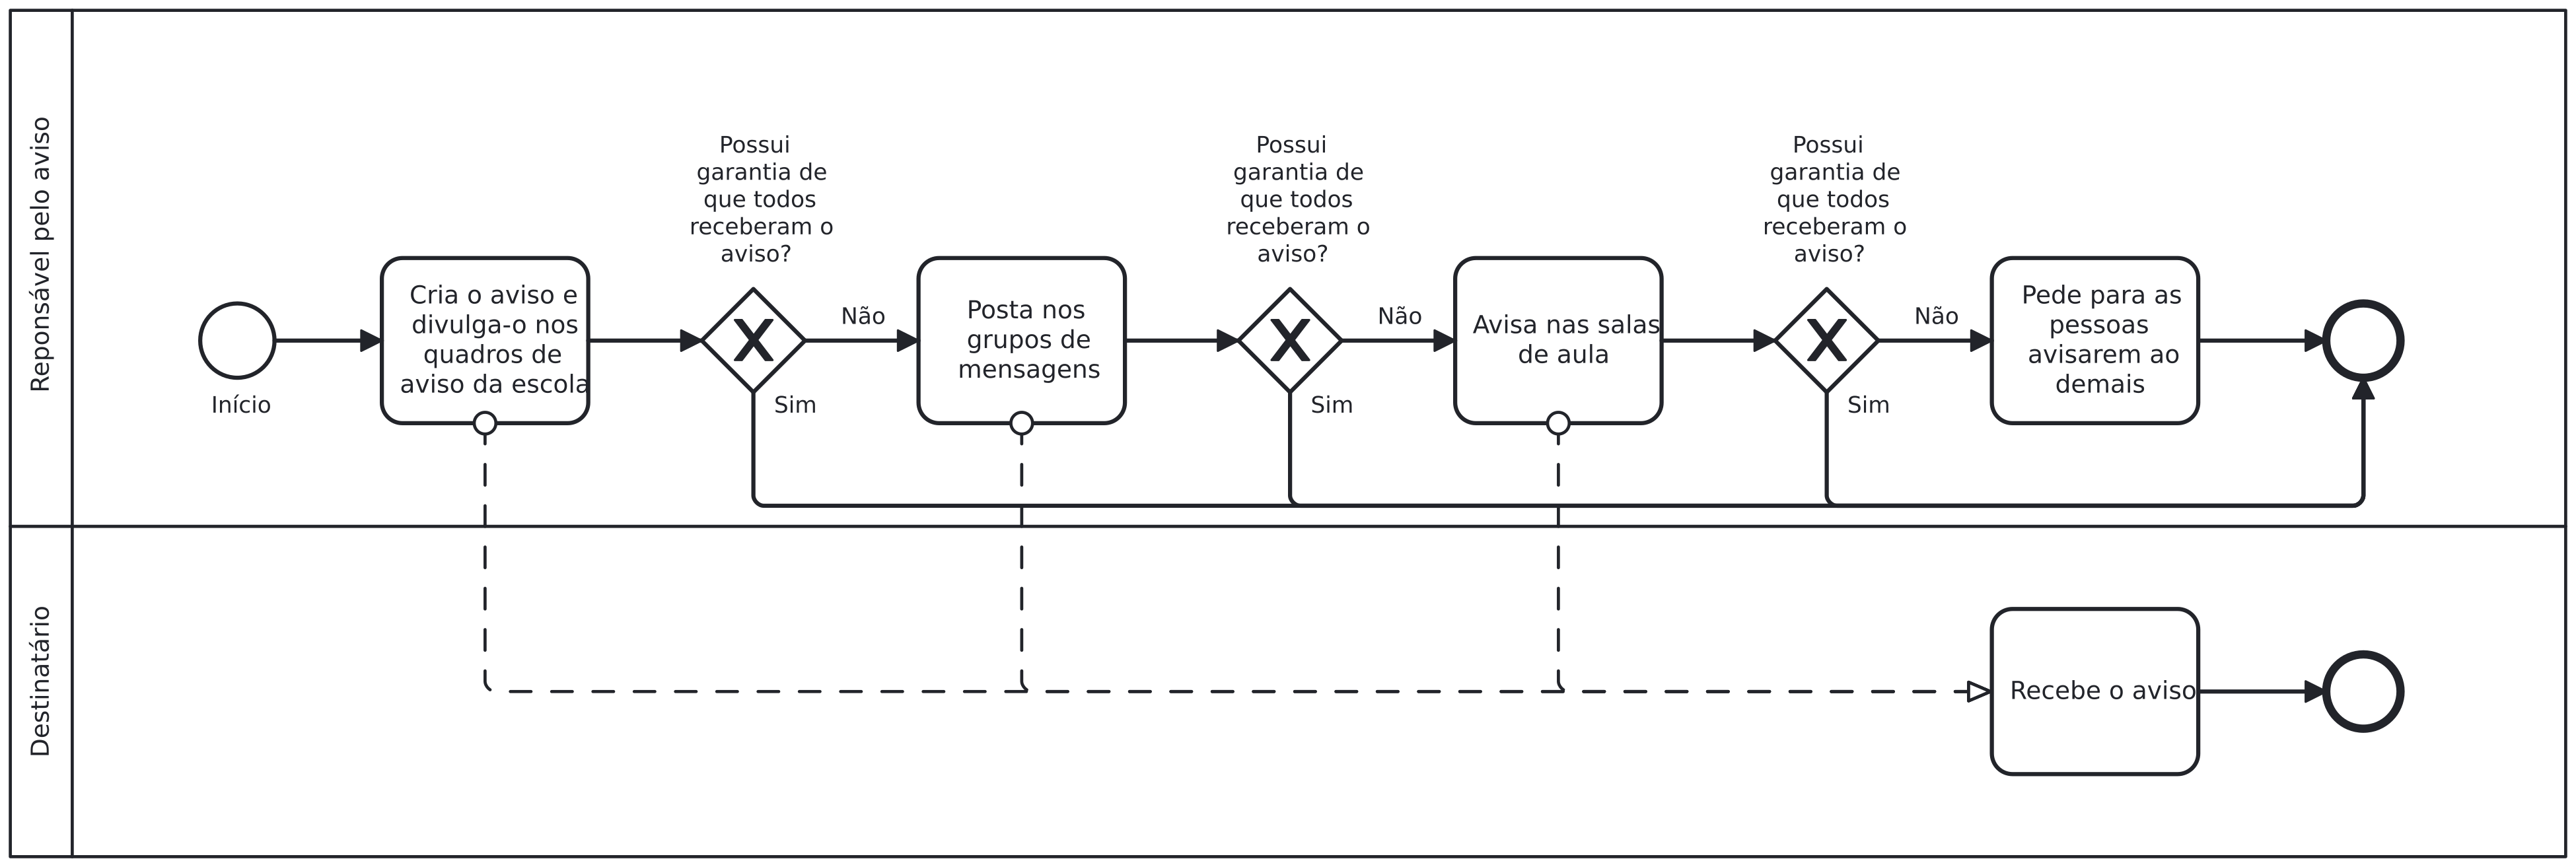
\includegraphics[width=\textwidth]{../../assets/diagram_as_is.png}
    \caption{Diagrama BPMN do processo atual (AS-IS) de comunicação escolar.}
    \label{fig:bpmn-asis}
\end{figure}

O fluxo atual apresenta a seguinte estrutura:

\begin{itemize}
    \item \textbf{Atores (raias):} o processo divide-se em duas raias: \textbf{Responsável pelo aviso} (quem elabora e propaga o comunicado) e \textbf{Destinatário} (quem recebe o aviso pelos canais utilizados).
    \item \textbf{Atividades e decisões:} a partir do evento de \textit{Início}, o \textit{Responsável pelo aviso} executa \textit{Cria o aviso e divulga-o nos quadros de aviso da escola}, enviando fluxo de mensagem ao \textit{Destinatário}. Em seguida, o gateway exclusivo \textit{Possui garantia de que todos receberam o aviso?} avalia o alcance: se \textit{Sim}, o fluxo encerra no evento de fim; se \textit{Não}, o responsável \textit{Posta nos grupos de mensagens} (com novo envio de mensagem ao destinatário) e passa por uma segunda decisão \textit{Possui garantia de que todos receberam o aviso?}. Caso ainda seja \textit{Não}, \textit{Avisa nas salas de aula} (com novo fluxo de mensagem ao destinatário) e avalia novamente em \textit{Possui garantia de que todos receberam o aviso?}. Persistindo a ausência de garantia (\textit{Não}), o responsável \textit{Pede para as pessoas avisarem ao demais} antes de alcançar o evento de fim. Na raia inferior, o \textit{Destinatário} apenas \textit{Recebe o aviso} e encerra seu fluxo.
    \item \textbf{Entradas e saídas:} entram no processo a necessidade de comunicar um aviso e seu conteúdo; saem do processo a divulgação escalonada por quadros físicos, grupos de mensagens, avisos em sala e repasse interpessoal, além do recebimento não rastreado pelo destinatário.
    \item \textbf{Problemas identificados:} o fluxo revela escalonamento manual por múltiplos meios na tentativa de suprir a falta de garantia de recebimento, retrabalho operacional, ausência de aprovação formal prévia antes da divulgação, falta de segmentação precisa por público, propagação informal via terceiros sem controle de integridade/relevância e inexistência de canal bidirecional estruturado para atendimento.
\end{itemize}

\section{Problemas e oportunidades de melhoria}

O Quadro~\ref{tab:melhorias-processo} correlaciona os problemas observados nas etapas do processo atual (AS-IS) aos seus impactos na rotina escolar e às melhorias incorporadas na evolução para o processo proposto (TO-BE).

\begin{longtable}{|p{3.0cm}|p{3.8cm}|p{3.8cm}|p{4.2cm}|}
\caption{Correlação entre problemas do processo AS-IS, impactos e melhorias propostas no processo TO-BE.} \label{tab:melhorias-processo} \\
\hline
\textbf{Etapa do processo} & \textbf{Problema identificado (AS-IS)} & \textbf{Impacto} & \textbf{Melhoria proposta (TO-BE)} \\
\hline
\endfirsthead
\hline
\textbf{Etapa do processo} & \textbf{Problema identificado (AS-IS)} & \textbf{Impacto} & \textbf{Melhoria proposta (TO-BE)} \\
\hline
\endhead
Criação e direcionamento do aviso & O aviso é criado e já divulgado diretamente no quadro de avisos da escola, sem definição estruturada prévia de público ou canais adequados e sem validação formal. & Exposição precoce ou irrelevante, ausência de governança sobre o conteúdo e necessidade de refazer a divulgação em outros meios quando o alcance é insuficiente. & Estruturar a criação em \textit{Criar o aviso ou comunicado}, \textit{Selecionar o público} e \textit{Selecionar os canais}, passando por \textit{Precisa de autorização?} com avaliação do \textit{Avaliador} (\textit{Avaliar a solicitação}, \textit{Comunicar aprovação} ou \textit{Comunicar a inviabilidade do aviso de forma motivada}, podendo chegar a \textit{Cancelar o aviso}). \\
\hline
Escalonamento entre canais e propagação informal & Diante da incerteza de alcance (\textit{Possui garantia de que todos receberam o aviso?}), o responsável replica manualmente em grupos de mensagens, avisa em salas de aula e pede que outras pessoas avisem aos demais. & Alto retrabalho, sobrecarga de mensagens, perda de avisos em grupos, dependência de presença física ou de repasse informal sujeito a ruído e perda de contexto. & Substituir o escalonamento manual em cascata pela publicação centralizada e segmentada em \textit{Enviar e/ou postar o aviso}, direcionando o comunicado aos \textit{Destinatários} pertinentes sem repasse informal por terceiros. \\
\hline
Recepção e ciência pelo destinatário & O \textit{Destinatário} apenas \textit{Recebe o aviso} de forma passiva por diferentes meios, sem mecanismo estruturado para registrar recebimento/leitura ou verificar o alcance completo. & Incerteza da escola sobre quem recebeu ou tomou ciência do aviso e dificuldade de acompanhamento por responsáveis com rotinas de trabalho. & Centralizar o recebimento em \textit{Receber o aviso, comunicado ou resposta} dentro da plataforma, associando a entrega ao público selecionado e viabilizando acompanhamento mais organizado da comunicação. \\
\hline
Comunicação e atendimento de demandas & Ausência de fluxo formal no processo atual para que responsáveis/tutores enviem mensagens à escola e recebam retorno documentado. & Trocas informais ou fragmentadas, ligações ou idas presenciais à escola e demora ou perda no direcionamento de dúvidas e solicitações. & Instituir fluxo formal iniciado pelo \textit{Tutor de aluno} (\textit{Criar uma mensagem} e \textit{Enviar a mensagem}), triado pelo \textit{Avaliador} (\textit{Distribuir a mensagem para o responsável}), avaliado pelo \textit{Respondente} (\textit{Avaliar a mensagem} e \textit{O respondente está correto?}, podendo \textit{Devolver a mensagem para redistribuição} ou \textit{Responder a mensagem}) e recebido em \textit{Receber resposta da menssagem}. \\
\hline
\end{longtable}

\section{Processo proposto — TO-BE}

O processo proposto (Figura~\ref{fig:bpmn-tobe}) reorganiza a comunicação escolar em cinco raias — \textbf{Tutor de aluno}, \textbf{Respondente (direção, coordenação, professor)}, \textbf{Avaliador (direção, coordenação, secretaria)}, \textbf{Emissor do aviso (direção, coordenação, professor)} e \textbf{Destinatários (tutor, comunidade escolar)} — substituindo o escalonamento manual e informal do AS-IS por fluxos definidos de publicação, moderação e atendimento.

\begin{figure}[H]
    \centering
    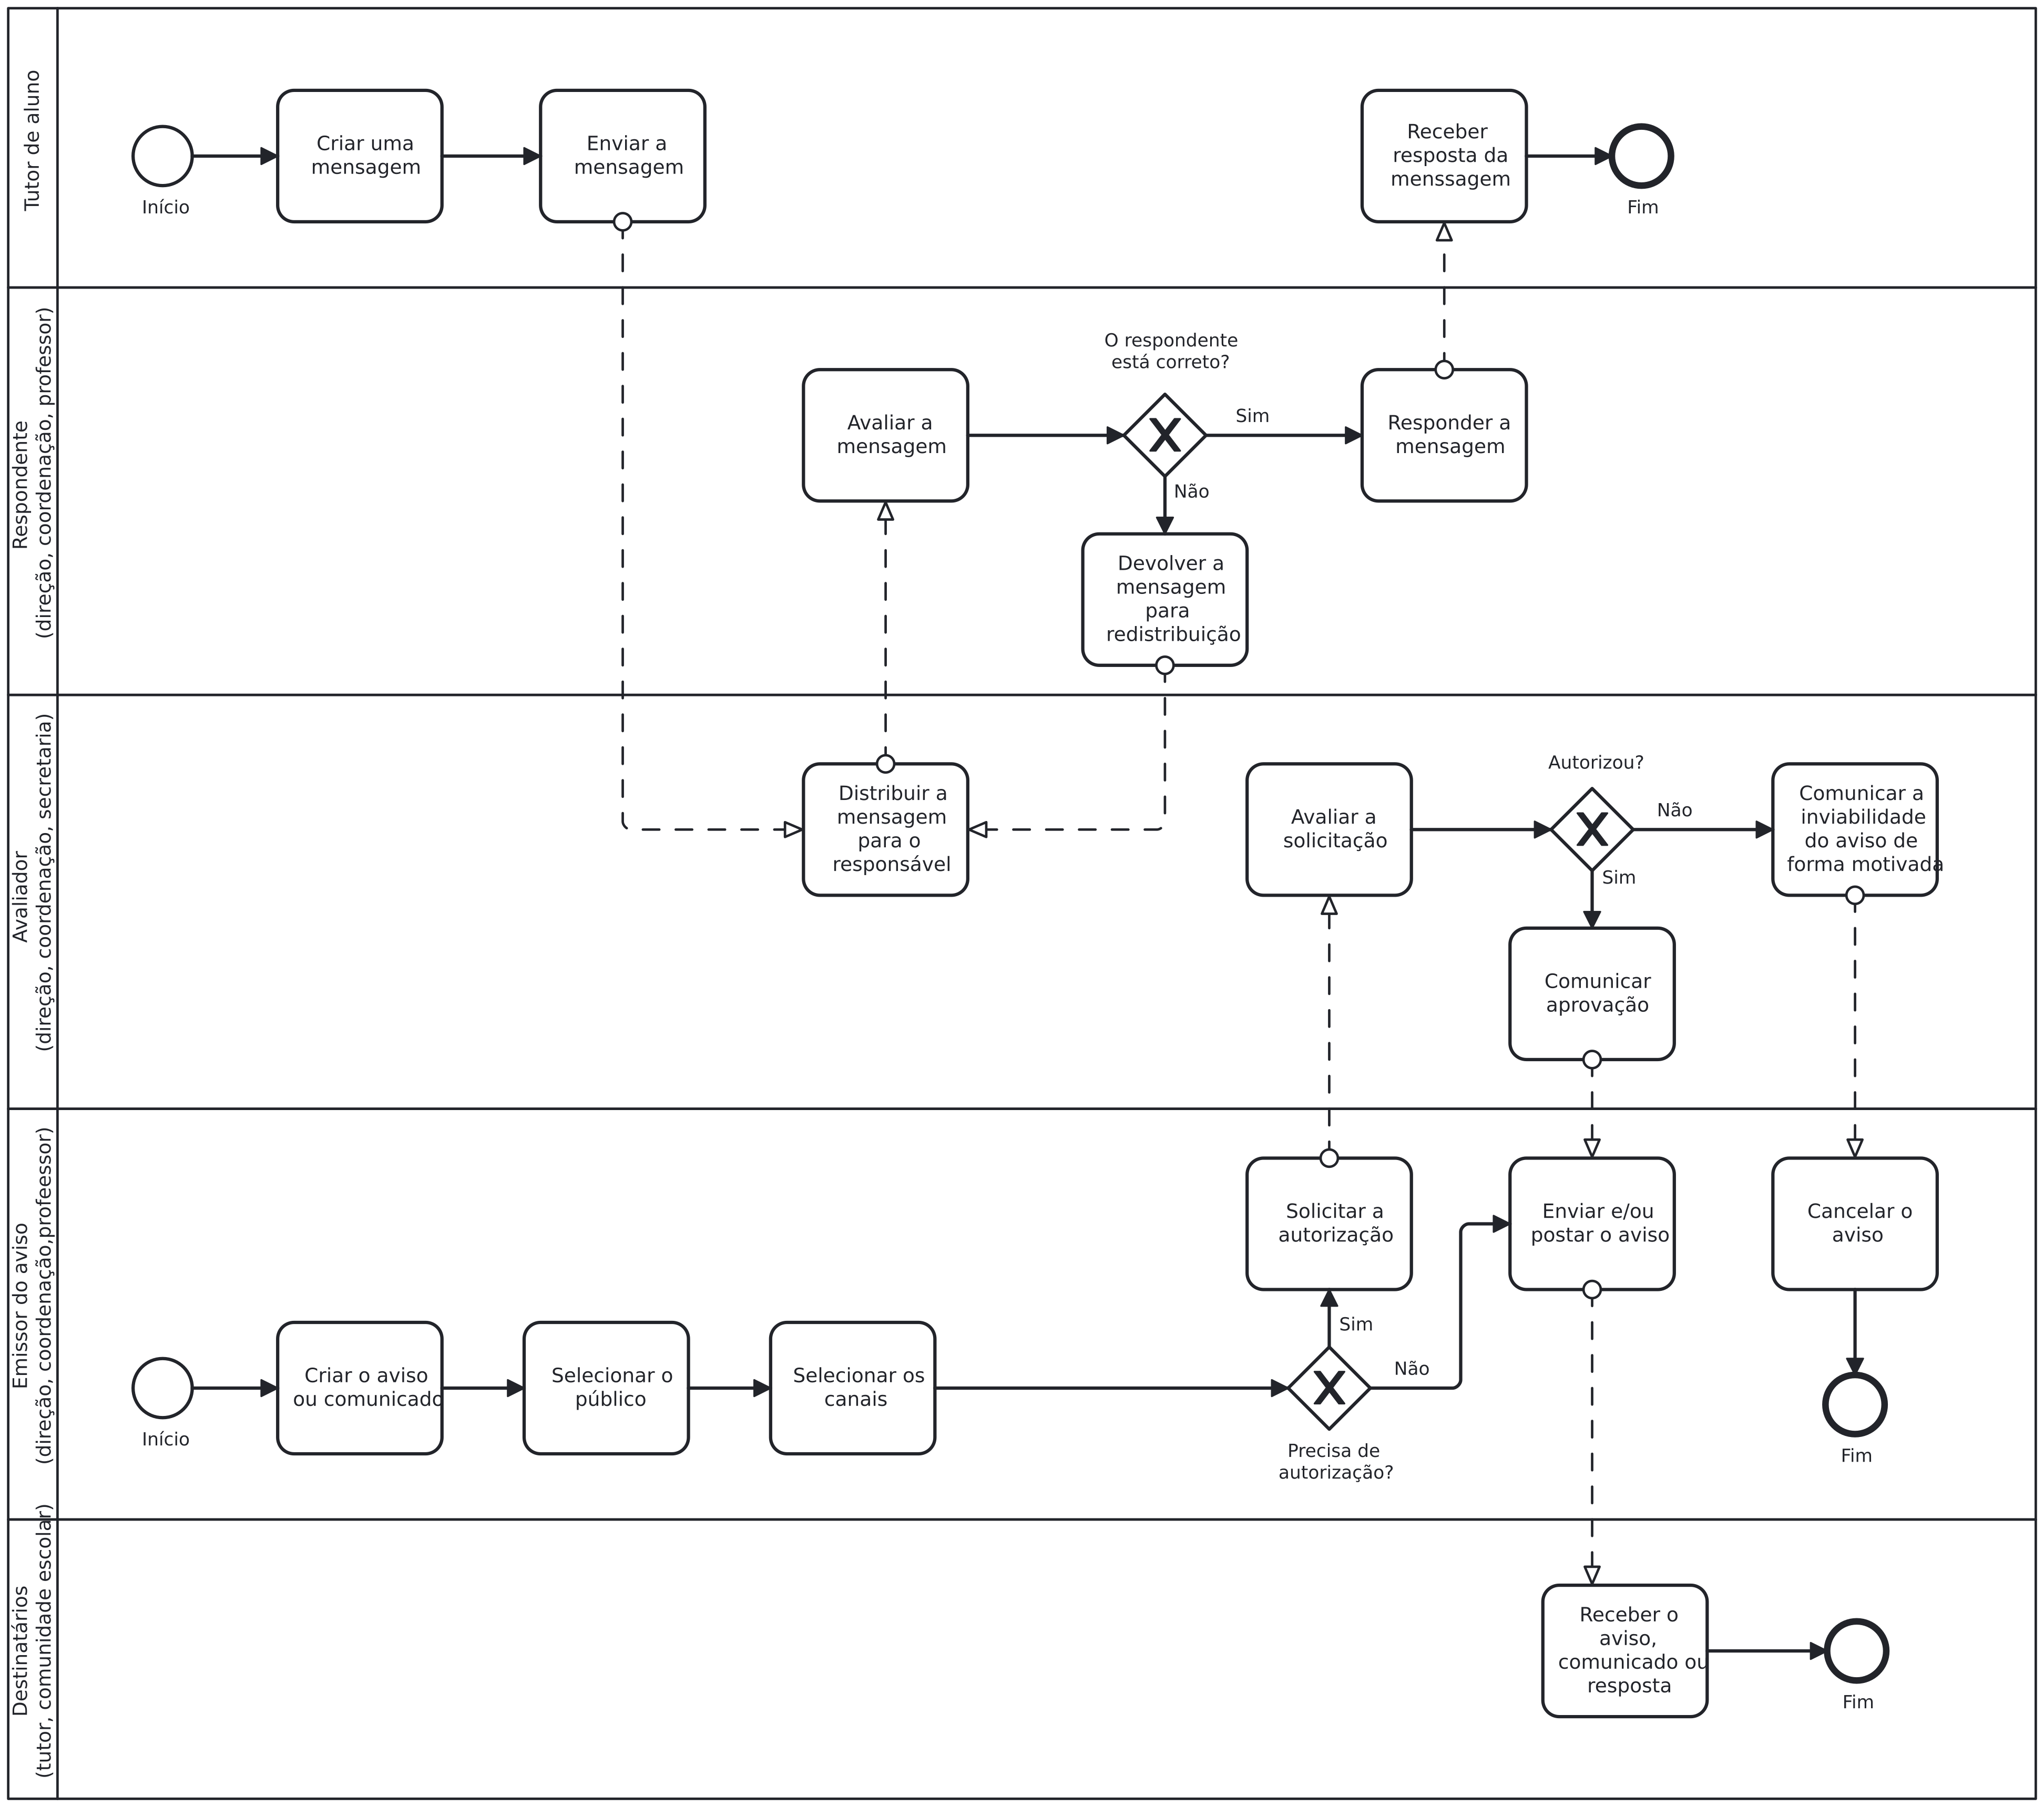
\includegraphics[width=\textwidth]{../../assets/diagrama_processo_v3.png}
    \caption{Diagrama BPMN do processo proposto (TO-BE) de comunicação escolar.}
    \label{fig:bpmn-tobe}
\end{figure}

A evolução em relação ao cenário atual ocorre por meio de dois fluxos, detalhados a seguir:

\begin{itemize}
    \item \textbf{Emissão, moderação e publicação de avisos:} o \textit{Emissor do aviso} executa \textit{Criar o aviso ou comunicado}, \textit{Selecionar o público} e \textit{Selecionar os canais}. No gateway \textit{Precisa de autorização?}, se a resposta for \textit{Sim}, o fluxo segue para \textit{Solicitar a autorização} ao \textit{Avaliador}, que realiza \textit{Avaliar a solicitação} e decide em \textit{Autorizou?}. Se \textit{Não}, o avaliador executa \textit{Comunicar a inviabilidade do aviso de forma motivada}, permitindo ao emissor \textit{Cancelar o aviso} e encerrar. Se \textit{Sim}, o avaliador executa \textit{Comunicar aprovação} (ou, quando a autorização prévia não é exigida, o emissor segue direto), viabilizando \textit{Enviar e/ou postar o aviso} para que os \textit{Destinatários} executem \textit{Receber o aviso, comunicado ou resposta}.
    \item \textbf{Envio, triagem e resposta de mensagens:} o \textit{Tutor de aluno} realiza \textit{Criar uma mensagem} e \textit{Enviar a mensagem}, que chega ao \textit{Avaliador} para \textit{Distribuir a mensagem para o responsável}. Na raia do \textit{Respondente}, ocorre \textit{Avaliar a mensagem} seguida do gateway \textit{O respondente está correto?}. Se \textit{Não}, o fluxo executa \textit{Devolver a mensagem para redistribuição} ao avaliador; se \textit{Sim}, o respondente executa \textit{Responder a mensagem}, fazendo com que o tutor realize \textit{Receber resposta da menssagem} e encerre o ciclo.
\end{itemize}

Em vez de repetir avisos em quadros físicos, grupos de mensagens, salas de aula e repasses informais sempre que falta garantia de recebimento, a escola passa a contar com validação prévia quando necessária, direcionamento por público e canais e um canal estruturado de atendimento com retorno rastreável.

\chapter{Especificação dos requisitos}

\section{Origem e rastreabilidade dos requisitos}

A especificação dos requisitos consolida as demandas levantadas no diagnóstico do cenário atual, no mapeamento de stakeholders, na visão sistêmica e na modelagem dos processos da solução, estabelecendo a rastreabilidade entre origem ou evidência, necessidade, requisito, classificação (funcional ou não funcional) e forma de verificação para orientar a concepção do sistema de quadro digital de avisos.

\begin{longtable}{|p{1.1cm}|p{2.5cm}|p{2.8cm}|p{3.4cm}|p{1.6cm}|p{3.0cm}|}
\caption{Matriz de origem e rastreabilidade dos requisitos funcionais.} \label{tab:requisitos-funcionais} \\
\hline
\textbf{ID} & \textbf{Origem / evidência} & \textbf{Necessidade} & \textbf{Requisito} & \textbf{Tipo} & \textbf{Como verificar?} \\
\hline
\endfirsthead
\hline
\textbf{ID} & \textbf{Origem / evidência} & \textbf{Necessidade} & \textbf{Requisito} & \textbf{Tipo} & \textbf{Como verificar?} \\
\hline
\endhead
RF01 & BPMN: Criar uma mensagem & Permitir que o tutor inicie o fluxo redigindo e registrando uma mensagem particular para a escola. & O sistema deve permitir que o tutor crie e envie uma mensagem com o conteúdo da demanda particular. & Funcional & Acessar o perfil de tutor, criar uma nova mensagem preenchendo os campos obrigatórios e enviá-la, verificando o registro de envio. \\
\hline
RF02 & BPMN: Criar o aviso ou comunicado & Permitir que os emissores registrem comunicados escolares preenchendo as informações e o conteúdo. & O sistema deve permitir que o emissor crie e salve um aviso ou comunicado institucional. & Funcional & Preencher os campos da tela de criação de aviso, salvar e conferir se o registro foi gerado corretamente. \\
\hline
RF03 & BPMN: Selecionar o público & Permitir direcionar o comunicado exatamente para os grupos ou salas de interesse. & O sistema deve permitir a seleção do público-alvo (tutores, alunos, turmas ou professores) para o aviso. & Funcional & Selecionar diferentes filtros de público na criação de aviso e verificar se a restrição de visualização é aplicada. \\
\hline
RF04 & BPMN: Selecionar os canais & Garantir que o aviso seja transmitido pelas vias adequadas. & O sistema deve permitir a seleção dos canais de divulgação do comunicado. & Funcional & Escolher canais específicos e validar se a configuração de entrega é registrada. \\
\hline
RF05 & BPMN: Distribuir a mensagem para o responsável & Encaminhar a mensagem criada pelo tutor ao setor competente (direção, coordenação ou professor). & O sistema deve permitir direcionar e distribuir a mensagem recebida para a fila do respondente adequado. & Funcional & Enviar uma mensagem como tutor e verificar se ela aparece na fila de distribuição para que o distribuidor encaminhe ao respondente correspondente. \\
\hline
RF06 & BPMN: Avaliar a solicitação & Permitir que o avaliador analise o pedido de publicação do aviso. & O sistema deve permitir que o avaliador visualize e avalie a solicitação de divulgação de um aviso. & Funcional & Acessar o painel do avaliador, abrir uma solicitação pendente de aviso e verificar as opções de decisão disponíveis. \\
\hline
RF07 & BPMN: Decisão Autorizou? (Sim/Não) & Verificar se o aviso foi aprovado pelo avaliador para seguir no fluxo. & O sistema deve direcionar o fluxo do aviso conforme o resultado da decisão de autorização (Sim/Não). & Funcional & Testar a aprovação e a rejeição de um aviso e verificar se o sistema encaminha corretamente para o próximo passo correspondente. \\
\hline
RF08 & BPMN: Comunicar a inviabilidade do aviso de forma motivada & Justificar e registrar a rejeição de avisos inviáveis para o emissor. & O sistema deve permitir registrar o motivo da inviabilidade e notificar o emissor sobre o indeferimento. & Funcional & Rejeitar um aviso informando uma justificativa e verificar se o status de inviabilidade é salvo e o emissor notificado. \\
\hline
RF09 & BPMN: Comunicar aprovação & Informar formalmente ao emissor que o aviso foi liberado. & O sistema deve emitir uma comunicação de aprovação para o emissor prosseguir com a postagem. & Funcional & Aprovar um aviso que requer autorização e verificar se a liberação é comunicada ao emissor. \\
\hline
RF10 & BPMN: Decisão Precisa de autorização? & Validar se o aviso gerado necessita de validação prévia antes de ser postado. & O sistema deve perguntar ao emissor do aviso se o aviso requer autorização. As regras sobre o que depende ou não de autorização são definidas pela escola em documento próprio e os emissores são obrigados a seguí-las. & Funcional & Submeter um aviso que exige aprovação e outro que dispensa, comprovando o desvio correto no fluxo. \\
\hline
RF11 & BPMN: Avaliar a mensagem & Permitir que o respondente analise a mensagem recebida do tutor e verifique a pertinência. & O sistema deve permitir que o respondente avalie a mensagem recebida do tutor. & Funcional & Abrir uma mensagem recebida na visão do respondente e registrar a avaliação inicial. \\
\hline
RF12 & BPMN: O respondente está correto? (Sim/Não) & Direcionar a mensagem para quem de direito ou devolvê-la caso tenha caído no setor errado. & O sistema deve permitir que o respondente responda diretamente (se correto) ou devolva a mensagem para redistribuição (se incorreto). & Funcional & Testar a devolução de uma mensagem para redistribuição e o atendimento direto, validando os desvios. \\
\hline
RF13 & BPMN: Devolver a mensagem para redistribuição & Reencaminhar a mensagem ao fluxo de triagem quando o respondente inicial não for o responsável. & O sistema deve retornar a mensagem para a fila de distribuição geral caso o respondente não seja o correto. & Funcional & Acionar a opção de devolução de mensagem e verificar se ela retorna para o painel de triagem. \\
\hline
RF14 & BPMN: Responder mensagem & Permitir que o respondente redija e envie a resposta definitiva ao tutor. & O sistema deve permitir ao respondente enviar a resposta estruturada para o tutor solicitante. & Funcional & Responder a uma mensagem como respondente e verificar se o conteúdo é entregue ao tutor. \\
\hline
RF15 & BPMN: Solicitar a autorização & Enviar o aviso para a fila de análise do avaliador quando necessário. & O sistema deve permitir submeter o aviso para a etapa de solicitação de autorização. & Funcional & Solicitar autorização para um aviso e checar se o item é encaminhado ao painel do avaliador. \\
\hline
RF16 & BPMN: Enviar e/ou postar o aviso & Publicar oficialmente o comunicado nos canais selecionados. & O sistema deve efetivar o envio e a publicação do aviso aprovado ou dispensado de autorização. & Funcional & Concluir o envio de um aviso e verificar se ele é disponibilizado com sucesso. \\
\hline
RF17 & BPMN: Cancelar o aviso & Interromper permanentemente o ciclo de um aviso que não será mais publicado. & O sistema deve permitir que o emissor cancele um aviso em elaboração ou inviabilizado. & Funcional & Acionar o cancelamento de um aviso e confirmar o encerramento do seu fluxo operacional. \\
\hline
RF18 & BPMN: Receber resposta da mensagem & Permitir que o tutor visualize a devolutiva enviada pela escola. & O sistema deve disponibilizar ao tutor a resposta oficial enviada pelo respondente. & Funcional & Acessar o perfil do tutor após a resposta e verificar a visualização da mensagem respondida. \\
\hline
RF19 & BPMN: Receber o aviso, comunicado ou resposta & Garantir que o público-alvo destinatário acesse o comunicado final divulgado. & O sistema deve disponibilizar o aviso publicado para consulta dos destinatários pertencentes ao público selecionado. & Funcional & Entrar com uma conta de destinatário e validar a recepção e visualização correta do aviso postado. \\
\hline
RNF01 & Seção 2.3 (Restrições e limitações); Seção 3.1 (Interfaces) & Garantir acesso ágil e notificações oportunas para a comunidade escolar, especialmente responsáveis em deslocamento ou rotina de trabalho. & A interface da aplicação deve priorizar o uso em dispositivos móveis e suportar mecanismos eficientes de notificação para novos avisos e respostas. & Não funcional & Testar a visualização, navegação e recebimento de notificações em telas de dispositivos móveis de diferentes tamanhos. \\
\hline
RNF02 & Seção 2.3 (Restrições e limitações); Seção 3.2 (Tabela~\ref{tab:ppdt}) & Impedir acessos indevidos a dados acadêmicos e ações de publicação ou aprovação de avisos fora do perfil autorizado. & O sistema deve aplicar controle de acesso baseado em perfil e vínculo institucional (direção, coordenação, secretaria, professores, alunos e responsáveis/tutores), restringindo consulta de dados, postagem e aprovação de avisos. & Não funcional & Executar testes de permissão com contas de cada perfil tentando acessar dados de outras turmas/alunos, postar ou aprovar avisos sem autorização. \\
\hline
RNF03 & Seção 3.3 (Quadro~\ref{tab:dicd}); Seção 4.2 (Quadro~\ref{tab:melhorias-processo}) & Assegurar confiabilidade na comunicação e evitar decisões baseadas em informações desatualizadas, incompletas ou sem ciência. & O sistema deve manter os registros de avisos, status de aprovação, respostas e eventos de entrega/leitura consistentes, íntegros e atualizados ao longo do fluxo. & Não funcional & Simular criação, moderação, leitura e resposta de registros e conferir se os estados e contagens permanecem coerentes e íntegros. \\
\hline
RNF04 & Seção 2.3 (Premissas e restrições); Seção 3.3 (Quadro~\ref{tab:dicd}) & Evitar sobrecarga de notificações e ruído de comunicação que comprometam a atenção aos avisos relevantes. & A apresentação e o envio de avisos devem respeitar critérios de relevância, categorização, segmentação por público e alinhamento ao calendário escolar. & Não funcional & Validar na interface e na lógica de exibição se avisos segmentados e datados aparecem apenas para o público e o período correspondentes. \\
\hline
RNF05 & Seção 3.3 (Dados, informação, conhecimento e decisão) & Coletar apenas os dados necessários à finalidade da comunicação e do acompanhamento escolar. & O sistema deve restringir a coleta e o armazenamento de dados ao estritamente necessário para o funcionamento dos fluxos de avisos, consulta autorizada e atendimento. & Não funcional & Inspecionar os campos exigidos nos formulários e entidades de dados e verificar se cada campo possui finalidade definida no escopo do sistema. \\
\hline
\end{longtable}

\section{Requisitos funcionais e não funcionais}

Para priorizar a concepção inicial do sistema, devem ser selecionados requisitos funcionais e requisitos não funcionais que cubram o núcleo operacional do quadro digital de avisos e do canal de atendimento, preservando as regras de negócio, permissões por perfil e restrições já estabelecidas no projeto. Os demais requisitos da matriz permanecem registrados para etapas subsequentes de evolução da solução. Recomenda-se a priorização dos seguinte requisito:

\subsection{Requisitos funcionais priorizáveis}

\begin{itemize}

    \item \textbf{RF01 — Criar uma mensagem:} permite que o tutor do aluno redija e envie uma mensagem com o conteúdo de dúvida, justificativa ou solicitação particular para a escola. \textit{Regras e restrições:} o envio deve ocorrer dentro do escopo de comunicação entre responsáveis/alunos e a escola, sem alterar os fluxos internos da secretaria.
    
    \item \textbf{RF02 — Criar o aviso ou comunicado:} permite que o emissor redija e salve um aviso ou comunicado institucional contendo as informações e o conteúdo necessários. \textit{Regras e restrições:} somente funcionários da escola podem criar e postar avisos, devendo respeitar as diretrizes institucionais, o calendário escolar e a pertinência do conteúdo para evitar ruído e sobrecarga de mensagens.
    
    \item \textbf{RF03 — Selecionar o público:} permite definir o público-alvo do aviso (como tutores, alunos, turmas ou professores) antes da divulgação. \textit{Regras e restrições:} a segmentação deve restringir a visualização aos destinatários pertinentes e respeitar a segregação de acesso por perfil e vínculo institucional.
    
    \item \textbf{RF06 / RF07 — Avaliar a solicitação e direcionar por decisão de autorização:} permite ao avaliador analisar a solicitação de divulgação de um aviso e direcionar o fluxo conforme a decisão de autorização (\textit{Sim} ou \textit{Não}). \textit{Regras e restrições:} somente direção, coordenação e secretaria podem aprovar avisos, cabendo a elas validar a adequação do comunicado antes da publicação e registrar motivação quando houver inviabilidade.
    
    \item \textbf{RF15 — Solicitar a autorização:} permite encaminhar o aviso elaborado para a fila de análise do avaliador quando a autorização prévia for aplicável. \textit{Regras e restrições:} a obrigatoriedade de moderação prévia segue as regras definidas pela escola em documento próprio ou, na modelagem inicial, a validação prévia quando exigida pela categoria/diretriz institucional.
    
    \item \textbf{RF16 — Enviar e/ou postar o aviso:} efetiva a publicação e o envio do aviso pelos canais selecionados após a aprovação ou quando dispensado de autorização prévia. \textit{Regras e restrições:} a publicação não deve depender de integração com sistemas administrativos, financeiros, de gestão de funcionários ou de matrículas, nem substituir os processos pedagógicos vigentes.
    
    \item \textbf{RF19 — Receber o aviso, comunicado ou resposta:} disponibiliza o comunicado publicado para consulta e recepção pelos destinatários pertencentes ao público selecionado. \textit{Regras e restrições:} cada usuário visualiza apenas os conteúdos autorizados para seu perfil e vínculo (alunos acessam apenas os próprios dados; responsáveis/tutores acessam dados de seus tutelados; professores acessam dados de suas turmas).
    
    \item \textbf{RF05 / RF14 — Distribuir a mensagem e responder ao tutor:} permite encaminhar a mensagem recebida do tutor ao respondente adequado (direção, coordenação ou professor) e viabiliza o envio da resposta oficial ao solicitante. \textit{Regras e restrições:} o atendimento deve respeitar a competência de cada perfil e manter o histórico registrado de forma organizada e tempestiva.
\end{itemize}

\subsection{Requisitos não funcionais priorizáveis}

\begin{itemize}
    \item \textbf{RNF01 — Priorização mobile e notificações:} a interface da aplicação deve priorizar o uso em dispositivos móveis e suportar mecanismos eficientes de notificação para novos avisos e respostas. \textit{Regras e restrições:} a entrega deve buscar tempestividade e relevância, evitando excesso de notificações e atendendo responsáveis com rotinas de trabalho ou deslocamento.
    
    \item \textbf{RNF02 — Controle de acesso baseado em perfil e vínculo:} o sistema deve impor segregação estrita de acesso, leitura, postagem e aprovação conforme o perfil e o vínculo institucional (direção, coordenação, secretaria, professores, alunos e responsáveis/tutores). \textit{Regras e restrições:} direção e coordenação acessam todos os dados; a secretaria acessa notas e frequências de todos os alunos; professores acessam apenas suas turmas; alunos acessam apenas seus próprios dados; responsáveis/tutores acessam dados de seus tutelados; apenas funcionários postam avisos; e somente direção, coordenação e secretaria aprovam comunicados.
    
    \item \textbf{RNF03 — Consistência, integridade e atualidade dos registros:} o sistema deve manter os registros de avisos, status de autorização, respostas e eventos de entrega/leitura consistentes, íntegros e atualizados ao longo do fluxo. \textit{Regras e restrições:} a coerência dos dados é condição para reduzir incertezas de recebimento e evitar decisões apoiadas em informações desatualizadas, incompletas ou inconsistentes.
\end{itemize}

\section{Histórias de usuário}

As histórias de usuário integram papéis, objetivos e benefícios para expressar necessidades e condições de qualidade de forma compreensível e verificável, conectando-se diretamente aos requisitos da matriz e preparando a definição dos cenários comportamentais da subseção seguinte. O Quadro~\ref{tab:historias-usuario} consolida as histórias correspondentes aos dezenove requisitos funcionais e aos cinco requisitos não funcionais da matriz.

\begin{longtable}{|p{3.8cm}|p{1.8cm}|p{4.2cm}|p{4.8cm}|}
\caption{Histórias de usuário vinculadas aos requisitos funcionais e não funcionais da matriz.} \label{tab:historias-usuario} \\
\hline
\textbf{História} & \textbf{Requisito} & \textbf{Descrição} & \textbf{Critério de aceitação} \\
\hline
\endfirsthead
\hline
\textbf{História} & \textbf{Requisito} & \textbf{Descrição} & \textbf{Critério de aceitação} \\
\hline
\endhead
Como tutor, quero criar e enviar uma mensagem com o conteúdo da demanda particular para a escola, para iniciar o atendimento de minhas solicitações. & RF01 & Inicia o fluxo de atendimento particular permitindo que o tutor redija e submeta sua mensagem à escola. & Mensagem enviada com campos obrigatórios preenchidos é registrada e encaminhada para triagem; campos obrigatórios vazios bloqueiam o envio e exibem alerta de validação. \\
\hline
Como emissor, quero criar e salvar um aviso ou comunicado institucional, para formalizar informações direcionadas à comunidade escolar. & RF02 & Registra o conteúdo e os dados iniciais de um aviso ou comunicado institucional para as etapas seguintes. & Registro salvo com título e texto fica disponível nas próximas etapas; o cancelamento da edição descarta dados não salvos e retorna à tela anterior. \\
\hline
Como emissor, quero selecionar o público-alvo para o aviso, para garantir que o comunicado atinja exatamente os grupos de interesse. & RF03 & Associa o aviso a grupos ou salas específicos (tutores, alunos, turmas ou professores). & Filtros selecionados vinculam o público-alvo à visualização do aviso; tentativa de salvar sem selecionar ao menos um grupo-alvo exibe solicitação de seleção. \\
\hline
Como emissor, quero selecionar os canais de divulgação do comunicado, para garantir que a mensagem seja transmitida pelas vias adequadas. & RF04 & Define e registra os canais pelos quais o comunicado será entregue. & Canais escolhidos ficam registrados na configuração de entrega; ausência de seleção de canal impede o salvamento e emite aviso correspondente. \\
\hline
Como distribuidor, quero direcionar e distribuir a mensagem recebida para a fila do respondente adequado, para que o setor competente realize o atendimento. & RF05 & Encaminha a mensagem recebida do tutor à fila do respondente correspondente ou trata casos sem definição clara de setor. & Mensagem encaminhada aparece na fila do respondente designado; mensagens com dados vagos permitem resposta direta do distribuidor informando a ocorrência. \\
\hline
Como avaliador, quero visualizar e avaliar a solicitação de divulgação de um aviso, para analisar o pedido de publicação. & RF06 & Abre e analisa uma solicitação de aviso pendente de autorização no painel do avaliador. & Solicitação pendente exibe detalhes e opções de decisão (aprovar ou rejeitar); item já avaliado e encerrado informa que não está mais pendente de análise. \\
\hline
Como sistema, quero direcionar o fluxo do aviso conforme o resultado da decisão de autorização, para seguir o caminho correto (Sim/Não). & RF07 & Encaminha o aviso para a etapa subsequente de acordo com a decisão registrada de autorização. & Decisão positiva encaminha para liberação e postagem; decisão negativa desvia para registro de inviabilidade e notificação do emissor. \\
\hline
Como avaliador, quero registrar o motivo da inviabilidade e notificar o emissor sobre o indeferimento. & RF08 & Registra a justificativa de recusa de um aviso inviável e informa o emissor. & Recusa com justificativa salva o status de inviabilidade e notifica o emissor; recusa sem justificativa obrigatória bloqueia a ação e exige o motivo. \\
\hline
Como sistema, quero emitir uma comunicação de aprovação para o emissor prosseguir com a postagem, para oficializar a liberação do aviso. & RF09 & Notifica formalmente o emissor quando o aviso é autorizado pelo avaliador. & Aprovação atualiza o status e emite aviso formal de liberação ao emissor; falha de rede registra erro e permite nova tentativa de notificação. \\
\hline
Como emissor, quero indicar se o aviso requer autorização prévia, para seguir as regras institucionais definidas pela escola. & RF10 & Registra o enquadramento do aviso quanto à necessidade de autorização prévia conforme as normas da escola. & Indicação direciona o fluxo para validação ou dispensa conforme a regra informada; omissão do critério exibe alerta solicitando a definição do status. \\
\hline
Como respondente, quero avaliar a mensagem recebida do tutor, para analisar a pertinência da demanda. & RF11 & Permite ao respondente abrir a mensagem recebida em sua fila e iniciar a análise de pertinência. & Abertura da mensagem registra visualização e início da avaliação; mensagem cancelada pelo remetente exibe aviso de chamado encerrado. \\
\hline
Como respondente, quero responder diretamente ou devolver a mensagem para redistribuição, para garantir que o setor correto atenda o tutor. & RF12 & Define o desvio de atendimento direto ou devolução à triagem conforme a competência sobre a demanda. & Respondente competente abre a interface de resposta ao tutor; respondente não competente aciona devolução para retorno à triagem. \\
\hline
Como sistema, quero retornar a mensagem para a fila de distribuição geral caso o respondente não seja o correto, para reorganizar o fluxo. & RF13 & Reencaminha à triagem geral as mensagens devolvidas por incorreção de setor ou responsável. & Devolução recoloca a mensagem na triagem geral como pendente de redistribuição; indisponibilidade da triagem armazena em fila de segurança e alerta o administrador. \\
\hline
Como respondente, quero enviar a resposta estruturada para o tutor solicitante, para solucionar a demanda apresentada. & RF14 & Registra e entrega ao tutor a resposta oficial elaborada pelo respondente. & Resposta preenchida é gravada e disponibilizada ao tutor; tentativa de envio com texto em branco bloqueia a conclusão e exige o campo de resposta. \\
\hline
Como emissor, quero submeter o aviso para a etapa de solicitação de autorização, para que o avaliador analise o conteúdo quando exigido. & RF15 & Envia o aviso para a fila do avaliador quando a autorização prévia é necessária. & Submissão encaminha o item ao painel do avaliador; tentativa de submeter rascunho inconsistente ou corrompido cancela o envio e aponta inconsistências. \\
\hline
Como sistema, quero efetivar o envio e a publicação do aviso aprovado ou dispensado de autorização, para disseminar a informação. & RF16 & Publica o comunicado nos canais configurados e o torna acessível ao público selecionado. & Postagem aprovada ou dispensada publica nos canais selecionados e exibe aos destinatários; falha de conexão encaminha para fila de reenvio automático e alerta o suporte. \\
\hline
Como emissor, quero cancelar um aviso em elaboração ou inviabilizado, para interromper permanentemente o seu ciclo operacional. & RF17 & Encerra definitivamente o ciclo de um aviso ainda em rascunho ou indeferido. & Cancelamento de aviso em elaboração ou inviabilizado encerra o fluxo e arquiva o registro; tentativa sobre aviso já publicado informa restrição e exige retificação. \\
\hline
Como tutor, quero visualizar a devolutiva enviada pela escola, para acompanhar o resultado da minha solicitação. & RF18 & Permite ao tutor consultar a resposta oficial emitida para sua demanda. & Resposta enviada aparece na aba de mensagens do tutor; consulta antes do retorno exibe o chamado com status pendente de atendimento. \\
\hline
Como destinatário, quero consultar o aviso publicado para o meu grupo, para ter acesso às informações direcionadas ao meu interesse. & RF19 & Exibe no feed do destinatário os comunicados publicados para os grupos aos quais pertence. & Avisos do público do usuário aparecem no feed; avisos direcionados a outros grupos permanecem ocultos da sua visualização. \\
\hline
Como usuário da comunidade escolar, quero acessar a plataforma e receber notificações de forma ágil em dispositivos móveis, para acompanhar avisos e respostas mesmo em deslocamento ou rotina de trabalho. & RNF01 & Assegura navegação responsiva e entrega oportuna de notificações em telas móveis sem sobrecarga indevida. & Interface adapta-se a diferentes tamanhos de tela móvel e entrega notificações de novos avisos e respostas em tempo oportuno, evitando ruído excessivo. \\
\hline
Como gestor ou membro da comunidade escolar, quero que o acesso a dados, postagens e aprovações respeite estritamente meu perfil e vínculo institucional, para proteger informações e manter a governança do sistema. & RNF02 & Aplica segregação por perfil e vínculo (direção, coordenação, secretaria, professores, alunos e responsáveis/tutores) em consultas, postagens e aprovações. & Cada perfil acessa apenas dados, turmas, tutelados ou ações autorizadas, bloqueando consultas indevidas e postagens ou aprovações fora das permissões definidas. \\
\hline
Como membro da comunidade escolar, quero que os registros de avisos, autorizações, respostas e leituras permaneçam consistentes, íntegros e atualizados, para confiar nas informações e apoiar decisões. & RNF03 & Garante coerência de estados, integridade dos registros e atualização contínua ao longo do fluxo. & Transições de estado, contagens e registros de leitura/resposta mantêm-se íntegros e atualizados após operações e consultas simultâneas. \\
\hline
Como destinatário ou emissor, quero que os avisos sejam exibidos e direcionados conforme relevância, categoria, público e calendário escolar, para evitar sobrecarga e perda de prazos. & RNF04 & Condiciona a exibição e o direcionamento dos avisos ao público-alvo, à categorização e ao período do calendário escolar. & Avisos segmentados e datados são exibidos apenas para o público correspondente e dentro do período válido no calendário escolar. \\
\hline
Como usuário e responsável pelo tratamento de dados, quero que o sistema colete e armazene apenas os dados necessários à finalidade da comunicação e do acompanhamento escolar, para preservar a privacidade e reduzir excessos. & RNF05 & Limita campos de entrada e armazenamento ao estritamente necessário para avisos, consultas autorizadas e atendimento. & Todos os campos de formulários e entidades possuem finalidade justificada no escopo do sistema, sem coleta de dados supérfluos ou não pertinentes. \\
\hline
\end{longtable}

\section{Cenários BDD}

Os cenários BDD (\textit{Behavior-Driven Development}) especificam o comportamento verificável do sistema por meio da estrutura \textit{Dado}, \textit{Quando} e \textit{Então}, detalhando tanto o fluxo principal (sucesso) quanto os fluxos alternativos ou de exceção associados às histórias de usuário e aos requisitos funcionais e não funcionais da matriz. O Quadro~\ref{tab:cenarios-bdd} consolida os cenários de aceitação elaborados para cada item.

\begin{longtable}{|p{1.6cm}|p{1.6cm}|p{3.6cm}|p{3.6cm}|p{4.0cm}|}
\caption{Cenários BDD (Dado/Quando/Então) vinculados aos requisitos e histórias de usuário.} \label{tab:cenarios-bdd} \\
\hline
\textbf{ID do cenário} & \textbf{RF/ História} & \textbf{Dado} & \textbf{Quando} & \textbf{Então} \\
\hline
\endfirsthead
\hline
\textbf{ID do cenário} & \textbf{RF/ História} & \textbf{Dado} & \textbf{Quando} & \textbf{Então} \\
\hline
\endhead
BDD01.1 & RF01 / HU01 & que o tutor está autenticado no sistema & ele preenche os campos obrigatórios da mensagem e aciona o botão de envio & a mensagem é registrada e encaminhada para a triagem da escola. \\
\hline
BDD01.2 & RF01 / HU01 & que o tutor está na tela de criação de mensagem & ele tenta enviar o formulário deixando campos obrigatórios em branco & o sistema exibe um alerta de validação e impede o envio até que sejam preenchidos. \\
\hline
BDD02.1 & RF02 / HU02 & que o emissor acessa a interface de criação de avisos & ele preenche o título, o texto do comunicado e salva o registro & o sistema armazena as informações com sucesso e disponibiliza o aviso para as etapas seguintes. \\
\hline
BDD02.2 & RF02 / HU02 & que o emissor está redigindo um aviso & ele clica no botão de cancelar a edição & o sistema descarta os dados não salvos e retorna à tela anterior. \\
\hline
BDD03.1 & RF03 / HU03 & que o emissor está configurando um aviso & ele seleciona turmas específicas ou perfis de destinatários e aplica a regra & o sistema vincula o público-alvo escolhido ao comunicado. \\
\hline
BDD03.2 & RF03 / HU03 & que o emissor tenta avançar sem selecionar nenhum grupo de destinatários & ele tenta salvar a configuração do público & o sistema exibe uma mensagem solicitando a seleção de ao menos um grupo-alvo. \\
\hline
BDD04.1 & RF04 / HU04 & que o emissor está definindo a distribuição de um aviso & ele seleciona canais específicos como WhatsApp ou painel de avisos e confirma & o sistema registra as preferências de entrega nos canais escolhidos. \\
\hline
BDD04.2 & RF04 / HU04 & que o emissor não seleciona um canal de comunicação disponível & ele tenta salvar a configuração de envio & o sistema emite um aviso informando a necessidade de informar os canais de comunicação. \\
\hline
BDD05.1 & RF05 / HU05 & que uma nova mensagem de tutor chegou ao sistema & o distribuidor analisa o teor e a encaminha para o respondente correspondente & a mensagem passa a constar na fila de atendimento do setor ou responsável designado. \\
\hline
BDD05.2 & RF05 / HU05 & que a mensagem recebida possui dados vagos que impedem a identificação do setor ou responsável pela resposta & o distribuidor tenta realizar o encaminhamento & o sistema permite que o distribuidor responda ao remetente diretamente informando a ocorrência. \\
\hline
BDD06.1 & RF06 / HU06 & que existe um aviso pendente aguardando autorização & o avaliador acessa seu painel e abre a solicitação & os detalhes do aviso e as opções de decisão (Aprovar ou Rejeitar) são exibidos. \\
\hline
BDD06.2 & RF06 / HU06 & que o avaliador tenta acessar uma solicitação que já foi avaliada e encerrada por outro usuário & ele abre o registro & o sistema informa que o item não está mais pendente de análise. \\
\hline
BDD07.1 & RF07 / HU07 & que o avaliador registrou uma decisão de autorização positiva (Sim) & o sistema processa a resposta & ele encaminha o aviso para a etapa de liberação e postagem. \\
\hline
BDD07.2 & RF07 / HU07 & que o avaliador registrou uma decisão negativa (Não) & o sistema processa a resposta & ele desvia o fluxo para o registro de inviabilidade e notificação do emissor. \\
\hline
BDD08.1 & RF08 / HU08 & que o avaliador rejeita um aviso informando a justificativa técnica & ele confirma a recusa & o sistema salva o status de inviabilidade e envia a notificação correspondente ao emissor. \\
\hline
BDD08.2 & RF08 / HU08 & que o avaliador tenta rejeitar um aviso sem preencher o campo de justificativa obrigatória & ele tenta concluir a recusa & o sistema bloqueia a ação e exige o preenchimento do motivo. \\
\hline
BDD09.1 & RF09 / HU09 & que o aviso foi devidamente autorizado pelo avaliador & o sistema atualiza o status do comunicado & ele envia um aviso formal de aprovação ao emissor para liberação da postagem. \\
\hline
BDD09.2 & RF09 / HU09 & que ocorre uma falha de comunicação na rede ao tentar emitir a aprovação & o sistema tenta notificar o emissor & ele gera um log de erro e permite re-tentar o envio da notificação. \\
\hline
BDD10.1 & RF10 / HU10 & que o emissor está finalizando a configuração do aviso & ele responde se o comunicado requer autorização com base nas normas da escola & o sistema direciona o fluxo para a validação ou dispensa a etapa conforme a regra informada. \\
\hline
BDD10.2 & RF10 / HU10 & que o emissor deixa de responder ao critério de autorização obrigatória & ele tenta avançar no cadastro & o sistema exibe um alerta solicitando a definição do status de autorização. \\
\hline
BDD11.1 & RF11 / HU11 & que uma mensagem foi encaminhada à fila do respondente & ele abre e lê o conteúdo da solicitação & o sistema registra que a mensagem foi visualizada e iniciada a avaliação de pertinência. \\
\hline
BDD11.2 & RF11 / HU11 & que o respondente tenta acessar uma mensagem que foi cancelada pelo remetente & ele clica no item & o sistema exibe uma mensagem de que o chamado foi encerrado. \\
\hline
BDD12.1 & RF12 / HU12 & que o respondente verifica que é o responsável pela demanda & ele seleciona a opção de atendimento direto & o sistema abre a interface de resposta ao tutor. \\
\hline
BDD12.2 & RF12 / HU12 & que o respondente verifica que a mensagem caiu no setor incorreto & ele seleciona a opção de devolução & o sistema envia a demanda de volta para a triagem. \\
\hline
BDD13.1 & RF13 / HU13 & que o respondente acionou a devolução por incorreção de setor ou de responsável & o sistema processa a ação & a mensagem retorna automaticamente para o painel de triagem geral com o status pendente de redistribuição. \\
\hline
BDD13.2 & RF13 / HU13 & que a triagem está temporariamente indisponível & o sistema tenta devolver a mensagem & ele armazena a solicitação em uma fila de segurança e notifica o administrador do sistema. \\
\hline
BDD14.1 & RF14 / HU14 & que o respondente preencheu o texto da resposta oficial & ele clica em enviar ao tutor & o sistema registra a resposta definitiva e a disponibiliza para o solicitante. \\
\hline
BDD14.2 & RF14 / HU14 & que o respondente tenta enviar uma resposta com o texto em branco & ele aciona o botão de envio & o sistema impede a conclusão e avisa que o campo de resposta é obrigatório. \\
\hline
BDD15.1 & RF15 / HU15 & que o aviso necessita de validação prévia & o emissor aciona o envio para autorização & o sistema encaminha o item para a fila do painel do avaliador. \\
\hline
BDD15.2 & RF15 / HU15 & que o emissor tenta solicitar autorização para um rascunho corrompido & ele clica no botão de submissão & o sistema cancela o envio e aponta inconsistências nos dados do aviso. \\
\hline
BDD16.1 & RF16 / HU16 & que um aviso foi aprovado pelo avaliador ou dispensado de autorização & o emissor confirma a postagem & o sistema publica o comunicado nos canais selecionados e o disponibiliza aos destinatários. \\
\hline
BDD16.2 & RF16 / HU16 & que ocorre uma falha de conexão com os canais de envio no momento da postagem & o sistema tenta publicar & ele armazena o aviso em uma fila de reenvio automático e alerta o suporte. \\
\hline
BDD17.1 & RF17 / HU17 & que o emissor decide não prosseguir com um aviso em rascunho ou recusado & ele aciona a opção de cancelamento do aviso & o sistema encerra o fluxo e arquiva o registro definitivamente. \\
\hline
BDD17.2 & RF17 / HU17 & que o emissor tenta cancelar um aviso que já foi totalmente publicado & ele clica em cancelar & o sistema exibe uma restrição informando que avisos publicados não podem ser cancelados diretamente, exigindo uma retificação. \\
\hline
BDD18.1 & RF18 / HU18 & que a escola respondeu à demanda do tutor & o tutor acessa seu perfil no sistema e abre a aba de mensagens & o sistema exibe a resposta oficial enviada pelo respondente. \\
\hline
BDD18.2 & RF18 / HU18 & que o tutor acessa o sistema antes de haver qualquer resposta da escola & ele consulta o histórico do chamado & o sistema exibe o status atual como pendente de atendimento. \\
\hline
BDD19.1 & RF19 / HU19 & que um aviso foi publicado para o público-alvo do qual o destinatário faz parte & o usuário entra com sua conta de destinatário no sistema & ele visualiza corretamente o comunicado postado em seu feed de avisos. \\
\hline
BDD19.2 & RF19 / HU19 & que o usuário pertence a um grupo que não foi selecionado como público-alvo do aviso & ele acessa o mural de comunicados & o sistema oculta aquele aviso específico de sua visualização. \\
\hline
BDD20.1 & RNF01 / HU20 & que um usuário autenticado acessa a aplicação por meio de um dispositivo móvel & ele navega pelo mural de avisos e recebe uma nova notificação & a interface ajusta-se adequadamente à tela móvel e exibe a notificação de forma oportuna. \\
\hline
BDD20.2 & RNF01 / HU20 & que o usuário acessa a aplicação em resolução reduzida de smartphone & ele abre formulários de criação de aviso ou resposta & todos os campos e botões permanecem legíveis e operáveis sem sobreposição de elementos. \\
\hline
BDD21.1 & RNF02 / HU21 & que um usuário autenticado possui perfil de professor vinculado apenas à turma A & ele consulta os dados acadêmicos disponíveis no sistema & o sistema exibe apenas os registros dos alunos da turma A, bloqueando o acesso às demais turmas. \\
\hline
BDD21.2 & RNF02 / HU21 & que um usuário autenticado possui perfil de aluno ou responsável/tutor & ele tenta acessar a funcionalidade de publicação ou aprovação de avisos & o sistema bloqueia a ação e nega o acesso por ausência de permissão do perfil. \\
\hline
BDD22.1 & RNF03 / HU22 & que um aviso passou por criação, aprovação, publicação e visualização por destinatários & o avaliador ou emissor consulta o histórico e o acompanhamento do comunicado & os status de moderação e os registros de entrega e leitura refletem fielmente as ações realizadas. \\
\hline
BDD22.2 & RNF03 / HU22 & que uma solicitação de tutor foi redistribuída e respondida pelo setor competente & o histórico do atendimento é consultado pelo tutor ou avaliador & o registro mantém a sequência íntegra e atualizada das movimentações e da resposta final. \\
\hline
BDD23.1 & RNF04 / HU23 & que um aviso foi categorizado e agendado conforme o calendário escolar para uma turma específica & um destinatário dessa turma acessa o sistema dentro do período vigente & o aviso é exibido com sua respectiva categoria durante o intervalo programado. \\
\hline
BDD23.2 & RNF04 / HU23 & que um aviso possui data de validade expirada no calendário escolar & um destinatário acessa o mural principal de avisos ativos & o sistema não exibe o comunicado expirado como aviso vigente, evitando ruído de informação. \\
\hline
BDD24.1 & RNF05 / HU24 & que um usuário preenche um formulário de cadastro de aviso ou de envio de mensagem & ele visualiza os campos solicitados pela interface & o sistema exige apenas os dados necessários à finalidade de comunicação, atendimento ou vínculo escolar. \\
\hline
BDD24.2 & RNF05 / HU24 & que o sistema armazena registros de comunicação e acompanhamento escolar & a estrutura de dados persistida é auditada quanto à finalidade & nenhum dado pessoal supérfluo ou estranho ao escopo da comunicação escolar é coletado ou armazenado. \\
\hline
\end{longtable}

\chapter{Modelagem dos dados}

\section{Descrição conceitual — MER}

A modelagem conceitual de dados estrutura os assuntos do domínio escolar sobre os quais o sistema precisa registrar informações, definindo as entidades, os atributos que as caracterizam, os identificadores que distinguem cada ocorrência e os relacionamentos expressos por verbos, articulados às regras de negócio e às dúvidas a validar no processo real. Esse modelo consolida as demandas dos requisitos funcionais e das informações necessárias à operação sem antecipar a representação gráfica visual.

O Quadro~\ref{tab:mer-entidades} apresenta as entidades conceituais do projeto, seu significado no domínio, seus identificadores e seus atributos principais (incluindo atributos de identificação, vínculo e controle presentes na modelagem).

\begin{longtable}{|p{3.0cm}|p{3.8cm}|p{2.3cm}|p{5.5cm}|}
\caption{Entidades, significado, identificadores e atributos principais do MER.} \label{tab:mer-entidades} \\
\hline
\textbf{Entidade} & \textbf{Significado} & \textbf{Identificador} & \textbf{Atributos principais} \\
\hline
\endfirsthead
\hline
\textbf{Entidade} & \textbf{Significado} & \textbf{Identificador} & \textbf{Atributos principais} \\
\hline
\endhead
PESSOA & Representa um indivíduo cadastrado no sistema, base para perfis institucionais e de acompanhamento. & id & usuario, email, nome, cpf, telefone, senha\_hash, nivel\_acesso\_id \\
\hline
ALUNO & Representa o estudante vinculado a uma pessoa para registro acadêmico e acompanhamento escolar. & pessoa\_id & pessoa\_id, matricula, serie \\
\hline
RESPONSAVEL & Representa o responsável ou tutor legal associado a uma pessoa para acompanhamento de alunos. & pessoa\_id & pessoa\_id, telefone\_emergencia \\
\hline
PARENTESCO & Representa o vínculo de parentesco ou responsabilidade entre um aluno e um responsável. & aluno\_id, responsavel\_id & aluno\_id, responsavel\_id, grau\_parentesco \\
\hline
FUNCIONARIO & Representa o membro da equipe escolar vinculado a uma pessoa para atuação e moderação. & pessoa\_id & pessoa\_id, registro\_funcional, tipo \\
\hline
NIVEL\_ACESSO & Define o perfil de permissão e as capacidades operacionais atribuídas aos usuários. & id & descricao, criar\_msm, dist\_msm, resp\_msm, criar\_aviso, aval\_aviso, rcb\_aviso \\
\hline
TURMA & Representa um grupamento escolar de alunos em determinado período de vigência. & id & nome, ano, sala, inicio\_vigencia, fim\_vigencia \\
\hline
DISCIPLINA & Representa uma matéria ou componente curricular do contexto escolar. & id & nome, codigo \\
\hline
ALUNO\_TURMA & Registra o vínculo e a situação de matrícula de um aluno em uma turma. & aluno\_id, turma\_id & aluno\_id, turma\_id, data\_matricula, status\_matricula \\
\hline
OFERTA\_ACADEMICA & Representa a oferta de uma disciplina a uma turma, com docente e programação de horários. & id & turma\_id, disciplina\_id, professor\_id, dias, turnos, horarios, hora\_inicio, hora\_fim \\
\hline
NOTA & Registra o resultado avaliativo obtido por um aluno em uma oferta acadêmica. & id & valor\_nota, nome\_avaliacao, data\_lancamento \\
\hline
FREQUENCIA & Registra a presença ou ausência de um aluno em atividade letiva de uma oferta acadêmica. & id & data\_aula, status\_presenca \\
\hline
AVISO & Representa um aviso ou comunicado institucional elaborado para divulgação na comunidade escolar. & id & autor\_id, titulo, descricao, formato, url, exige\_autorizacao, nivel\_urgencia, data\_criacao, data\_publicacao, status \\
\hline
AVISO\_SEGMENTACAO & Define os critérios ou alvos específicos de segmentação de um aviso. & id & aviso\_id, tipo\_alvo, alvo\_id \\
\hline
MENSAGEM & Representa uma mensagem particular, dúvida, justificativa ou solicitação trocada no sistema. & id & remetente\_id, destinatario\_id, titulo, descricao, formato, url, tipo, data\_criacao, status \\
\hline
RESPOSTA\_MENSAGEM & Registra a resposta emitida em resposta a uma mensagem. & id & mensagem\_id, titulo, descricao, data\_criacao \\
\hline
AUTORIZACAO\_AVISO & Registra a análise, a decisão e o parecer de autorização de um aviso. & id & aviso\_id, avaliador\_id, data\_solicitacao, data\_avaliacao, status, feedback \\
\hline
ENVIO & Registra a efetivação do envio de um aviso por canal e critério de segmentação. & id & aviso\_id, data\_envio, canal, tipo\_segmentacao \\
\hline
VISUALIZACAO & Registra a visualização ou ciência de um item por uma pessoa. & aviso\_id, pessoa\_id & aviso\_id, pessoa\_id, data\_hora\_visualizacao \\
\hline
REACAO\_AVISO & Registra a reação de uma pessoa a um aviso publicado. & aviso\_id, pessoa\_id & aviso\_id, pessoa\_id, tipo \\
\hline
COMENTARIO & Registra um comentário associado a um aviso. & id & texto, data\_criacao \\
\hline
\end{longtable}

Os relacionamentos entre essas entidades são formulados por meio de verbos que expressam a associação no domínio, acompanhados das regras de negócio e definições a confirmar junto à realidade escolar:

\begin{itemize}
    \item \textbf{Nível de Acesso} \textit{define} \textbf{Pessoa}: define permissões específicas (como criar ou distribuir mensagens, criar ou avaliar avisos e visualizar o \textit{feed}) para cada nível de acesso.
    \item \textbf{Responsável} \textit{possui} \textbf{Parentesco}: indica o vínculo de responsabilidade de um responsável; exige confirmar o grau de parentesco exato e quantos responsáveis um aluno pode ter vinculados simultaneamente.
    \item \textbf{Aluno} \textit{possui} \textbf{Parentesco}: associa o aluno ao vínculo de parentesco; requer confirmar como o sistema valida esse vínculo e a responsabilidade legal pelo aluno.
    \item \textbf{Funcionário} \textit{orienta} \textbf{Turma}: indica a orientação de turma por funcionário; exige confirmar se um funcionário (como professor orientador) pode orientar mais de uma turma no mesmo período letivo.
    \item \textbf{Aluno} \textit{matricula} \textbf{Aluno\_Turma}: associa o aluno ao registro de matrícula na turma; requer confirmar como registrar o histórico de turmas anteriores e o status do aluno (matriculado, desmatriculado, transferido ou concluído).
    \item \textbf{Turma} \textit{engloba} \textbf{Aluno\_Turma}: agrupa os vínculos de matrícula da turma; exige confirmar a capacidade máxima de alunos permitida por turma em cada ano letivo.
    \item \textbf{Turma} \textit{possui} \textbf{Oferta Acadêmica}: relaciona a turma às ofertas que compõem sua grade; requer confirmar a estrutura de disciplinas, dias da semana, turnos e horários associados.
    \item \textbf{Disciplina} \textit{compoe} \textbf{Oferta Acadêmica}: vincula a disciplina às ofertas em que é ministrada; exige confirmar se a mesma disciplina pode ser ofertada múltiplas vezes para a mesma turma em horários diferentes.
    \item \textbf{Funcionário} \textit{ministra} \textbf{Oferta Acadêmica}: indica a atuação docente na oferta; requer confirmar se um professor pode lecionar a mesma oferta em conjunto com outro docente ou se há apenas um responsável por oferta.
    \item \textbf{Oferta Acadêmica} \textit{registra} \textbf{Nota}: vincula os lançamentos avaliativos à oferta acadêmica; exige confirmar critérios de lançamento, etapas de avaliação permitidas e pesos por atividade.
    \item \textbf{Aluno} \textit{recebe} \textbf{Nota}: associa as notas ao aluno; requer confirmar como o aluno e seus responsáveis consultam o boletim e as notas parciais lançadas pelo professor.
    \item \textbf{Oferta Acadêmica} \textit{controla} \textbf{Frequência}: vincula os registros de frequência à oferta acadêmica; exige confirmar se o lançamento ocorre por aula diária ou horário ou se é consolidado por período ou dia letivo.
    \item \textbf{Aluno} \textit{acumula} \textbf{Frequência}: associa os registros de presença e ausência ao aluno; requer confirmar o cálculo da porcentagem de presença mínima obrigatória e o registro de faltas justificadas.
    \item \textbf{Funcionário} \textit{cria} \textbf{Aviso}: indica a autoria do aviso por funcionário; exige confirmar quais categorias de funcionários têm autonomia para criar avisos institucionais e quais exigem moderação prévia.
    \item \textbf{Aviso} \textit{segmenta} \textbf{Aviso\_Segmentação}: associa o aviso aos critérios de direcionamento; requer confirmar se um aviso pode ser direcionado simultaneamente a múltiplas turmas, séries específicas ou a toda a escola.
    \item \textbf{Aviso} \textit{pode\_requerer} \textbf{Autorização Aviso}: indica a submissão condicional do aviso à autorização; exige confirmar se todo aviso criado exige aprovação prévia de um avaliador (diretor ou coordenador) antes da liberação.
    \item \textbf{Funcionário} \textit{avalia} \textbf{Autorização Aviso}: indica a análise do pedido de autorização pelo funcionário avaliador; exige confirmar se o avaliador pode retornar o aviso com \textit{feedback} para correções do autor antes da aprovação final.
    \item \textbf{Pessoa} \textit{envia} \textbf{Mensagem}: registra a origem do envio de mensagens; requer confirmar como funciona o fluxo de envio e direcionamento de dúvidas ou mensagens diretas entre usuários.
    \item \textbf{Pessoa} \textit{recebe} \textbf{Mensagem}: registra o recebimento da mensagem pelo destinatário; requer confirmar se o destinatário recebe notificações em tempo real ao ser acionado em uma nova mensagem.
    \item \textbf{Mensagem} \textit{possui} \textbf{Resposta Mensagem}: associa as respostas à mensagem original; exige confirmar se há árvore de respostas encadeadas ou apenas fluxo linear de réplica.
    \item \textbf{Aviso} \textit{gera} \textbf{Envio}: vincula o aviso aos registros de envio; requer confirmar quais canais de transmissão (notificação no aplicativo, portal, e-mail) são acionados automaticamente na publicação.
    \item \textbf{Aviso} \textit{compoe} \textbf{Reação Aviso}: vincula as reações ao aviso publicado; requer confirmar quais tipos de reações (curtidas, \textit{emojis}) os usuários podem registrar.
    \item \textbf{Pessoa} \textit{compoe} \textbf{Reação Aviso}: vincula a reação à pessoa que a registrou; requer confirmar se cada usuário registra apenas uma reação por aviso ou pode alterá-la posteriormente.
    \item \textbf{Aviso} \textit{compoe} \textbf{Comentario}: vincula os comentários ao aviso; requer confirmar se os comentários passam por moderação prévia antes de ficarem visíveis aos demais usuários.
    \item \textbf{Pessoa} \textit{compoe} \textbf{Comentario}: vincula o comentário à pessoa autora; requer confirmar quem tem permissão para excluir comentários inadequados em um aviso institucional.
    \item \textbf{Pessoa} \textit{recebe} \textbf{Visualização}: associa a visualização à pessoa; requer confirmar como é registrado o carimbo de data e hora para comprovar a leitura de um aviso obrigatório.
    \item \textbf{Aviso} \textit{registra} \textbf{Visualização}: associa as visualizações ao aviso; requer confirmar se o sistema gera relatórios consolidados para a diretoria indicando quem visualizou ou deixou de visualizar o aviso.
\end{itemize}

\section{Representação gráfica — DER}

O Diagrama Entidade-Relacionamento (DER) apresentado na Figura~\ref{fig:der-modelo} traduz o modelo conceitual descrito no MER (Seção~\ref{sec:mer}), representando as entidades, seus respectivos atributos e identificadores, bem como os relacionamentos e as cardinalidades mínimas e máximas que expressam as regras de negócio do domínio escolar. Para a representação gráfica, adotou-se a notação de Peter Chen, na qual as entidades são representadas por retângulos, os relacionamentos por losangos associados aos respectivos verbos e os atributos por elipses conectadas às suas entidades.

\begin{figure}[H]
    \centering
    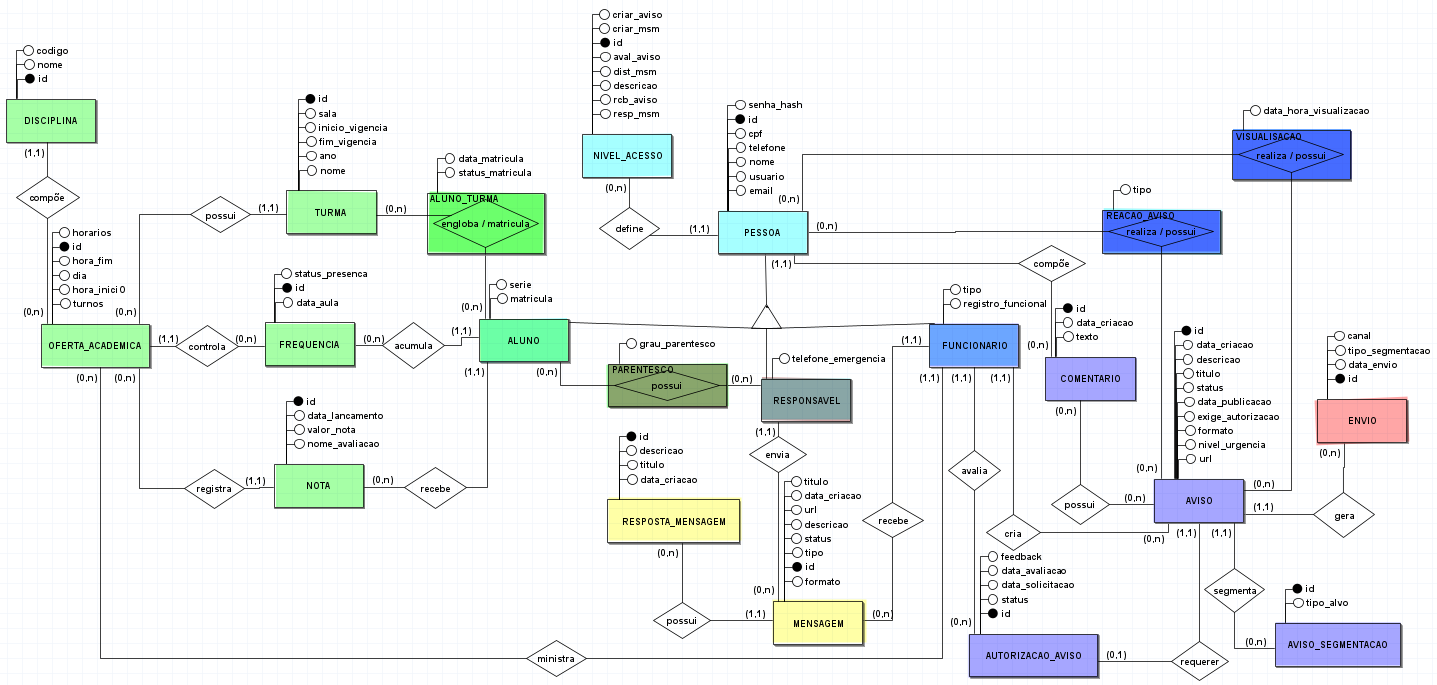
\includegraphics[width=\textwidth]{../../assets/der.png}
    \caption{Diagrama Entidade-Relacionamento (DER) do sistema em notação Peter Chen.}
    \label{fig:der-modelo}
\end{figure}

A leitura do diagrama apresenta a organização dos dados em quatro núcleos principais integrados, que refletem a estrutura do domínio escolar e as funcionalidades do sistema:

\begin{itemize}
    \item \textbf{Identidade, perfis e vínculos familiares:} a entidade \textbf{PESSOA} centraliza os dados cadastrais básicos e se especializa em \textbf{ALUNO}, \textbf{RESPONSAVEL} e \textbf{FUNCIONARIO}, associando-se a \textbf{NIVEL\_ACESSO} (cardinalidade $(1,1)$ de pessoa para $(0,n)$ de nível de acesso) para definição das permissões operacionais, enquanto \textbf{PARENTESCO} formaliza a relação entre responsáveis e alunos.
    \item \textbf{Estrutura acadêmica e acompanhamento escolar:} \textbf{TURMA} e \textbf{DISCIPLINA} compõem \textbf{OFERTA\_ACADEMICA} (ministrada por \textbf{FUNCIONARIO}), enquanto \textbf{ALUNO\_TURMA} vincula os estudantes às turmas vigentes e os registros de \textbf{NOTA} e \textbf{FREQUENCIA} associam o desempenho e a assiduidade de cada aluno às respectivas ofertas acadêmicas.
    \item \textbf{Comunicação institucional, moderação e engajamento:} \textbf{FUNCIONARIO} cria \textbf{AVISO}, que se relaciona com \textbf{AVISO\_SEGMENTACAO} para direcionamento por público-alvo, com \textbf{AUTORIZACAO\_AVISO} (avaliada por funcionário habilitado) quando há necessidade de aprovação prévia, com \textbf{ENVIO} para registro dos canais acionados e com \textbf{VISUALIZACAO}, \textbf{REACAO\_AVISO} e \textbf{COMENTARIO} para acompanhamento de ciência e interação dos usuários.
    \item \textbf{Atendimento e troca de mensagens:} \textbf{PESSOA} atua tanto no envio quanto no recebimento de \textbf{MENSAGEM}, que pode possuir registros associados em \textbf{RESPOSTA\_MENSAGEM} para documentar a devolutiva oficial da escola ao solicitante.
\end{itemize}

\section{Regras e validação do modelo}

A validação do modelo conceitual busca explicar os relacionamentos mais relevantes e suas cardinalidades, além de verificar a correspondência entre os dados modelados, os requisitos especificados e os processos do sistema.

\subsection{Relacionamentos relevantes e cardinalidades}

Os principais relacionamentos do modelo organizam os perfis, a estrutura acadêmica, a comunicação institucional e o atendimento às demandas da comunidade escolar, com cardinalidades que refletem as regras do domínio:

\begin{itemize}
    \item \textbf{Perfis, vínculos e permissões:} \textbf{NIVEL\_ACESSO} define as permissões de \textbf{PESSOA} (cada pessoa possui um nível de acesso, enquanto um nível de acesso pode associar-se a várias pessoas). \textbf{PESSOA} especializa-se em \textbf{ALUNO}, \textbf{RESPONSAVEL} e \textbf{FUNCIONARIO} conforme o papel institucional, e o vínculo familiar entre \textbf{ALUNO} e \textbf{RESPONSAVEL} é formalizado por \textbf{PARENTESCO}.
    \item \textbf{Organização acadêmica e acompanhamento:} \textbf{ALUNO} vincula-se a \textbf{TURMA} por meio de \textbf{ALUNO\_TURMA} (relação muitos-para-muitos associativa), e \textbf{TURMA}, \textbf{DISCIPLINA} e \textbf{FUNCIONARIO} articulam-se em \textbf{OFERTA\_ACADEMICA} (e na orientação de turma), servindo de base para os registros de \textbf{NOTA} e \textbf{FREQUENCIA} vinculados ao aluno e à oferta.
    \item \textbf{Emissão, autorização, segmentação e envio de avisos:} \textbf{FUNCIONARIO} cria \textbf{AVISO}, que pode exigir moderação em \textbf{AUTORIZACAO\_AVISO} (um aviso pode ter zero, uma ou mais solicitações de autorização ao longo de seu ciclo de revisão, vinculadas a um avaliador). A segmentação do público ocorre por \textbf{AVISO\_SEGMENTACAO}, e a distribuição é registrada em \textbf{ENVIO} (um aviso pode gerar um ou mais envios conforme canais e segmentações).
    \item \textbf{Engajamento e atendimento:} \textbf{AVISO} e \textbf{PESSOA} associam-se a \textbf{VISUALIZACAO}, \textbf{REACAO\_AVISO} e \textbf{COMENTARIO} para registrar leitura e interação, enquanto \textbf{PESSOA} envia e recebe \textbf{MENSAGEM}, que pode ter registros associados em \textbf{RESPOSTA\_MENSAGEM} para formalizar a devolutiva.
\end{itemize}

\subsection{Correspondência entre dados, requisitos e processo}

Para validar se o modelo de dados sustenta o que foi especificado nos requisitos e modelado nos fluxos do processo, o Quadro~\ref{tab:correspondencia-mer} cruza os requisitos funcionais com as entidades e atributos correspondentes e aponta as regras ou definições que ainda precisam ser confirmadas na prática escolar.

\begin{longtable}{|p{3.4cm}|p{4.8cm}|p{6.4cm}|}
\caption{Correspondência entre requisitos funcionais, dados do modelo e pontos de confirmação.} \label{tab:correspondencia-mer} \\
\hline
\textbf{Requisito / necessidade} & \textbf{Dados e entidades} & \textbf{Regra ou ponto a confirmar} \\
\hline
\endfirsthead
\hline
\textbf{Requisito / necessidade} & \textbf{Dados e entidades} & \textbf{Regra ou ponto a confirmar} \\
\hline
\endhead
\textbf{RF01:} Criar e enviar mensagem particular do tutor & \textbf{MENSAGEM} (\texttt{remetente\_id}, \texttt{destinatario\_id}, \texttt{titulo}, \texttt{descricao}, \texttt{tipo}, \texttt{data\_criacao}, \texttt{status}) & Confirmar o direcionamento inicial da demanda particular para o setor responsável. \\
\hline
\textbf{RF02:} Criar e salvar aviso ou comunicado & \textbf{AVISO} (\texttt{autor\_id}, \texttt{titulo}, \texttt{descricao}, \texttt{formato}, \texttt{status}, \texttt{data\_criacao}) & Confirmar quais categorias ou situações exigem aprovação prévia pela escola. \\
\hline
\textbf{RF03:} Selecionar público-alvo do aviso & \textbf{AVISO\_SEGMENTACAO}, \textbf{TURMA}, \textbf{ALUNO}, \textbf{ALUNO\_TURMA}, \textbf{OFERTA\_ACADEMICA} & Validar como a segmentação por turma ou série alcança os alunos e responsáveis vinculados. \\
\hline
\textbf{RF04:} Selecionar canais de divulgação & \textbf{ENVIO} (\texttt{canal}, \texttt{data\_envio}, \texttt{tipo\_segmentacao}) & Confirmar quais canais de notificação e divulgação serão efetivamente integrados. \\
\hline
\textbf{RF05:} Distribuir mensagem para o respondente adequado & \textbf{MENSAGEM} (\texttt{remetente\_id}, \texttt{destinatario\_id}, \texttt{status}) & Definir como o sistema identifica ou encaminha a mensagem ao respondente competente. \\
\hline
\textbf{RF06:} Visualizar e avaliar solicitação de aviso & \textbf{AUTORIZACAO\_AVISO} (\texttt{aviso\_id}, \texttt{avaliador\_id}, \texttt{status}) & Confirmar quais papéis possuem permissão formal para avaliar solicitações. \\
\hline
\textbf{RF07:} Direcionar fluxo conforme decisão de autorização & \textbf{AUTORIZACAO\_AVISO} (\texttt{status}, \texttt{feedback}) & Verificar se a aprovação leva diretamente à publicação ou a nova etapa de envio. \\
\hline
\textbf{RF08:} Registrar motivo da inviabilidade e notificar emissor & \textbf{AUTORIZACAO\_AVISO} (\texttt{feedback}, \texttt{status}); \textbf{AVISO} (\texttt{status}) & Definir como registrar e comunicar de forma motivada o indeferimento ao autor. \\
\hline
\textbf{RF09:} Emitir comunicação de aprovação & \textbf{AUTORIZACAO\_AVISO} (\texttt{status}); \textbf{AVISO} (\texttt{status}) & Confirmar se a comunicação de aprovação ocorre no sistema, por notificação ou ambos. \\
\hline
\textbf{RF10:} Indicar se o aviso requer autorização prévia & \textbf{AVISO} (\texttt{exige\_autorizacao}); \textbf{NIVEL\_ACESSO} & Confirmar se a exigência de autorização decorre do nível de acesso, da categoria ou de regra da escola. \\
\hline
\textbf{RF11:} Avaliar mensagem recebida do tutor & \textbf{MENSAGEM}, \textbf{VISUALIZACAO} & Confirmar se há necessidade de registrar data e hora da análise inicial pelo respondente. \\
\hline
\textbf{RF12:} Responder diretamente ou devolver mensagem & \textbf{MENSAGEM} (\texttt{status}) & Definir o registro simples do desvio entre responder diretamente e devolver para redistribuição. \\
\hline
\textbf{RF13:} Retornar mensagem para fila de distribuição geral & \textbf{MENSAGEM} (\texttt{status} de redistribuição) & Confirmar para qual fila ou painel a mensagem retorna quando devolvida. \\
\hline
\textbf{RF14:} Enviar resposta estruturada ao tutor & \textbf{RESPOSTA\_MENSAGEM} (\texttt{mensagem\_id}, \texttt{titulo}, \texttt{descricao}, \texttt{data\_criacao}) & Confirmar se o atendimento encerra na resposta do respondente ou permite réplicas encadeadas. \\
\hline
\textbf{RF15:} Submeter aviso para solicitação de autorização & \textbf{AUTORIZACAO\_AVISO}, \textbf{AVISO} (\texttt{status}) & Verificar se a submissão para análise bloqueia temporariamente a edição pelo autor. \\
\hline
\textbf{RF16:} Efetivar envio e publicação do aviso & \textbf{ENVIO}, \textbf{AVISO} (\texttt{status} publicado) & Confirmar se o sistema prevê agendamento de publicação para datas futuras. \\
\hline
\textbf{RF17:} Cancelar aviso em elaboração ou inviabilizado & \textbf{AVISO} (\texttt{status} cancelado) & Definir em quais estados do ciclo de vida o cancelamento é permitido. \\
\hline
\textbf{RF18:} Disponibilizar resposta oficial ao tutor & \textbf{RESPOSTA\_MENSAGEM}, \textbf{MENSAGEM} & Confirmar se o tutor recebe alerta imediato quando a resposta é disponibilizada. \\
\hline
\textbf{RF19:} Garantir consulta do aviso pelo público-alvo & \textbf{VISUALIZACAO}, \textbf{REACAO\_AVISO}, \textbf{COMENTARIO}, \textbf{NOTA}, \textbf{FREQUENCIA} & Confirmar a obrigatoriedade do registro de leitura/ciência para avisos críticos. \\
\hline
\end{longtable}

\chapter{Concepção da solução e prototipação}

\section{Visão da solução}

A solução proposta consiste em uma aplicação de comunicação e acompanhamento escolar, concebida com abordagem \textit{mobile-first} e suporte a acesso \textit{web}, voltada a instituições de ensino básico. Sua arquitetura funcional organiza os fluxos definidos no processo TO-BE em torno de dois eixos principais — a divulgação moderada e segmentada de avisos/comunicados e o canal estruturado de mensagens e atendimento —, além da consulta de informações acadêmicas (notas e frequências) sem interferir nos sistemas administrativos internos ou na gestão da secretaria.

\begin{itemize}
    \item \textbf{Usuários e perfis:} a plataforma atende aos papéis mapeados na comunidade escolar — \textbf{Emissor do aviso} (direção, coordenação e professores), \textbf{Avaliador} (direção, coordenação e secretaria), \textbf{Distribuidor / triagem}, \textbf{Respondente} (direção, coordenação e professores), \textbf{Tutor / responsável legal}, \textbf{Aluno} e \textbf{Destinatários} —, com permissões condicionadas ao nível de acesso e ao vínculo institucional.
    \item \textbf{Principais funcionalidades:} criação e salvamento de avisos; definição de público-alvo (turmas, perfis ou vínculos) e canais de divulgação; submissão e avaliação de autorização com registro de aprovação ou indeferimento motivado; publicação e exibição segmentada no mural; registro de visualização/ciência; consulta de notas, frequências e declarações conforme o perfil; e envio, triagem, eventual devolução para redistribuição e resposta oficial a mensagens.
    \item \textbf{Interfaces:} telas responsivas priorizando dispositivos móveis, compostas por feed/mural de avisos segmentados, formulário de criação e configuração de comunicados, painel de avaliação e moderação, caixa de entrada e fila de atendimento de mensagens e visão de acompanhamento acadêmico.
    \item \textbf{Fluxo geral de uso:} na comunicação institucional, o emissor elabora o aviso, define público e canais e, quando exigido pelas regras escolares, submete à avaliação antes da publicação para os destinatários autorizados. No atendimento, o tutor envia uma mensagem particular, que passa pela triagem para o respondente competente; caso o setor não seja o correto, a mensagem pode retornar para redistribuição até a emissão da resposta oficial visualizada pelo tutor.
\end{itemize}

\section{Protótipos de interface}

Os protótipos de interface ilustram as interações centrais do sistema em telas de uso móvel, conectando cada tela ao perfil de usuário, aos requisitos funcionais atendidos e à sua finalidade operacional. O Quadro~\ref{tab:prototipos-interface} sintetiza os protótipos previstos e indica as respectivas figuras, apresentadas em sequência a seguir.

\begin{longtable}{|p{2.9cm}|p{2.5cm}|p{2.2cm}|p{6.8cm}|}
\caption{Relação entre protótipos de interface, perfis de usuário, requisitos associados e finalidades.} \label{tab:prototipos-interface} \\
\hline
\textbf{Tela / Protótipo} & \textbf{Usuário} & \textbf{RF associado} & \textbf{Finalidade} \\
\hline
\endfirsthead
\hline
\textbf{Tela / Protótipo} & \textbf{Usuário} & \textbf{RF associado} & \textbf{Finalidade} \\
\hline
\endhead
Tela de Login \newline (Figura~\ref{fig:tela-login}) & Todos os usuários & RF01 a RF19 & Permitir autenticação segura e direcionamento para o painel de funcionalidades conforme perfil e vínculo. \\
\hline
Criação de aviso \newline (Figura~\ref{fig:tela-criacao-aviso}) & Emissor do aviso & RF02, RF03, RF04, RF10, RF15, RF16, RF17 & Permitir redigir o comunicado, selecionar público-alvo e canais, indicar necessidade de autorização e submeter, publicar ou cancelar o aviso. \\
\hline
Avaliação de avisos \newline (Figura~\ref{fig:tela-avaliacao-aviso}) & Avaliador & RF06, RF07, RF08, RF09 & Exibir solicitações pendentes de autorização para aprovar ou indeferir com justificativa motivada e disparar a comunicação ao emissor. \\
\hline
Mural de avisos \newline (Figura~\ref{fig:tela-mural-avisos}) & Destinatário (tutor, aluno, comunidade) & RF19 & Apresentar apenas os avisos publicados direcionados ao perfil/vínculo do usuário e registrar a consulta e ciência do comunicado. \\
\hline
Envio de mensagem particular \newline (Figura~\ref{fig:tela-envio-mensagem}) & Tutor do aluno & RF01, RF18 & Permitir redigir e enviar dúvidas, justificativas ou solicitações à escola e acompanhar o status e a resposta oficial recebida. \\
\hline
Triagem de mensagens \newline (Figura~\ref{fig:tela-triagem-mensagens}) & Distribuidor e Respondente & RF05, RF11, RF12, RF13, RF14 & Encaminhar mensagens recebidas à fila adequada, avaliar pertinência, devolver para redistribuição quando incorreto ou enviar resposta oficial. \\
\hline
Resposta de mensagem \newline (Figura~\ref{fig:tela-resposta-mensagem}) & Respondente (direção, coordenação, professor) & RF14, RF18 & Permitir redigir e enviar a resposta oficial à mensagem recebida, registrando o envio e a visualização pelo tutor. \\
\hline
\end{longtable}

\begin{figure}[H]
    \centering
    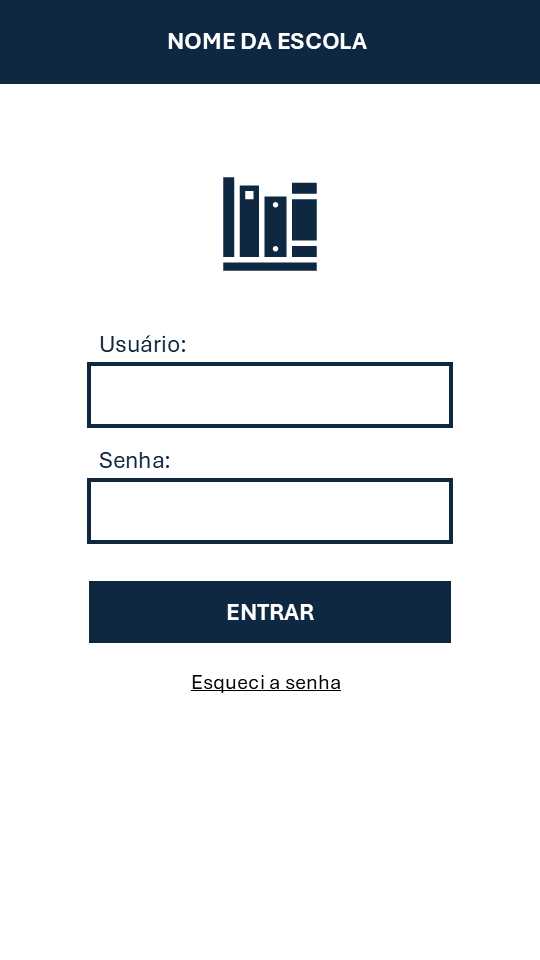
\includegraphics[height=0.35\textheight,keepaspectratio]{../../assets/telas/Slide1.PNG}
    \caption{Tela de Login.}
    \label{fig:tela-login}
\end{figure}

\begin{figure}[H]
    \centering
    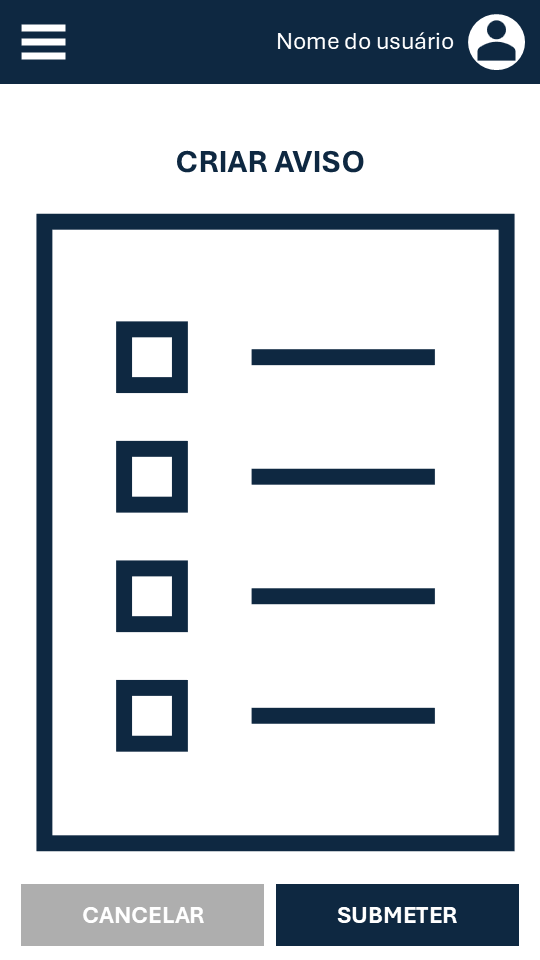
\includegraphics[height=0.35\textheight,keepaspectratio]{../../assets/telas/Slide2.PNG}
    \caption{Tela de criação e segmentação de aviso.}
    \label{fig:tela-criacao-aviso}
\end{figure}

\begin{figure}[H]
    \centering
    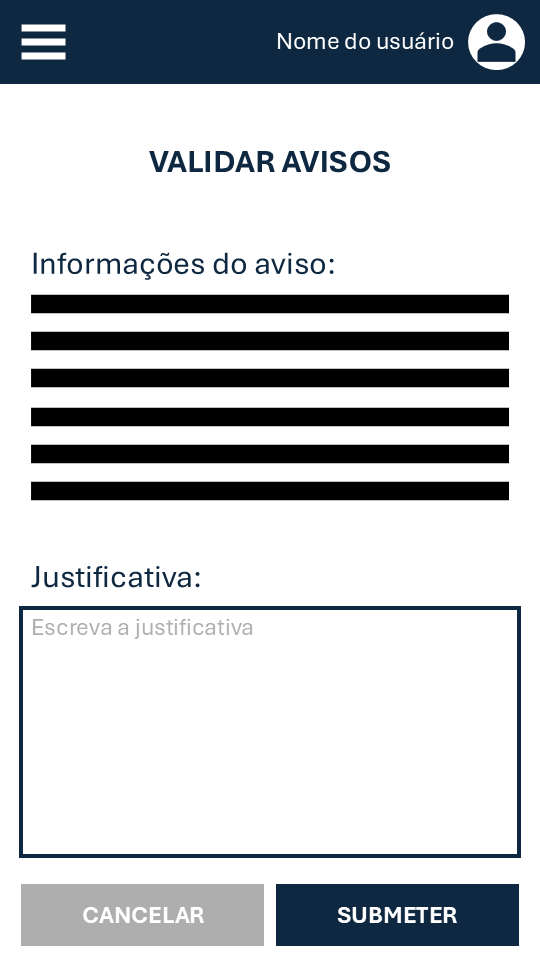
\includegraphics[height=0.35\textheight,keepaspectratio]{../../assets/telas/Slide3.PNG}
    \caption{Tela de avaliação de avisos.}
    \label{fig:tela-avaliacao-aviso}
\end{figure}

\begin{figure}[H]
    \centering
    
\includegraphics[height=0.35\textheight,keepaspectratio]{../../assets/telas/Slide4.PNG}
    \caption{Tela do mural de avisos.}
    \label{fig:tela-mural-avisos}
\end{figure}

\begin{figure}[H]
    \centering
    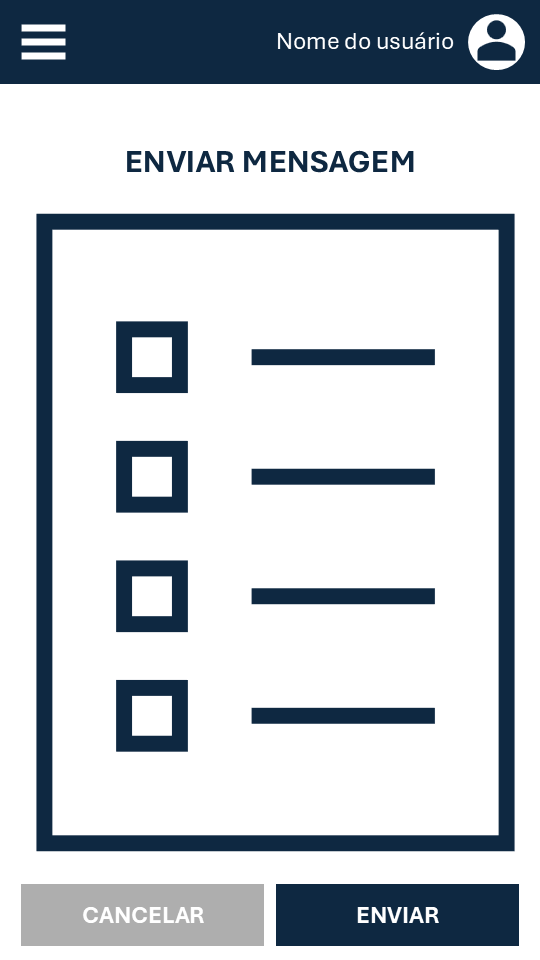
\includegraphics[height=0.35\textheight,keepaspectratio]{../../assets/telas/Slide5.PNG}
    \caption{Tela de envio de mensagem particular.}
    \label{fig:tela-envio-mensagem}
\end{figure}

\begin{figure}[H]
    \centering
    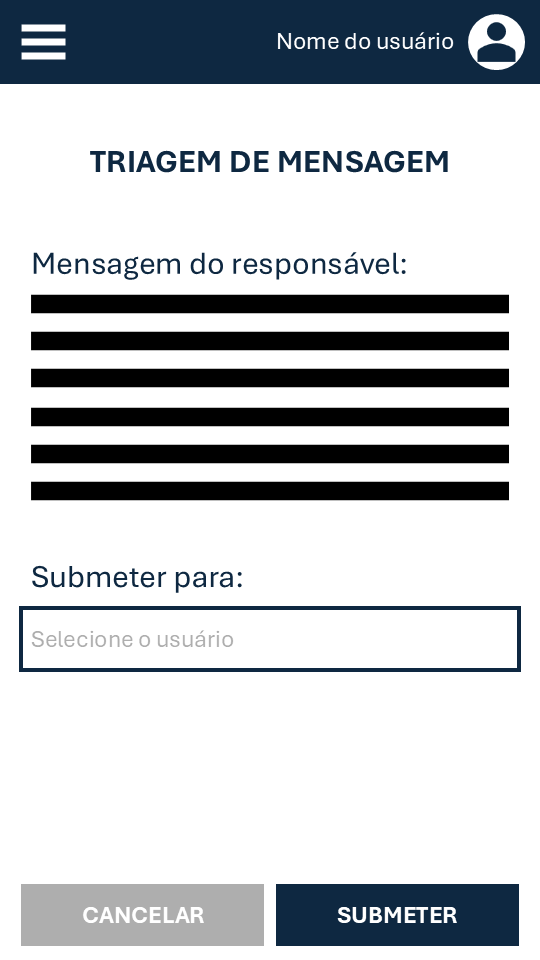
\includegraphics[height=0.35\textheight,keepaspectratio]{../../assets/telas/Slide6.PNG}
    \caption{Tela de triagem de mensagens.}
    \label{fig:tela-triagem-mensagens}
\end{figure}

\begin{figure}[H]
    \centering
    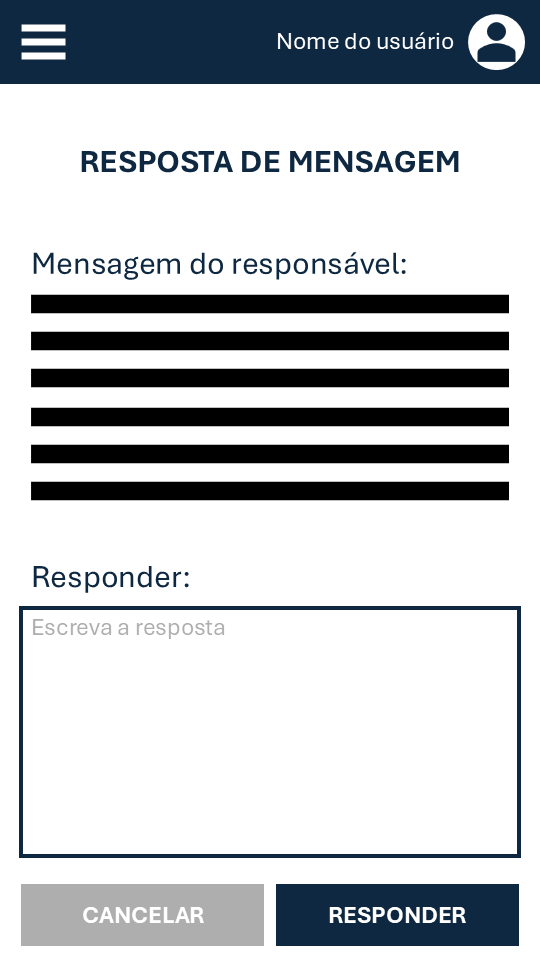
\includegraphics[height=0.35\textheight,keepaspectratio]{../../assets/telas/Slide7.PNG}
    \caption{Tela de resposta de mensagem.}
    \label{fig:tela-resposta-mensagem}
\end{figure}

\section{Privacidade, segurança e qualidade da informação}

A concepção da solução incorpora mecanismos de proteção de dados, controle de acesso e qualidade informacional coerentes com o modelo de dados e com os requisitos do projeto:

\begin{itemize}
    \item \textbf{Dados pessoais tratados e minimização:} o sistema trata dados cadastrais e de vínculo institucional de pessoas (\textbf{PESSOA}, \textbf{ALUNO}, \textbf{RESPONSAVEL}, \textbf{FUNCIONARIO}, \textbf{PARENTESCO}), registros de comunicação e atendimento (\textbf{AVISO}, \textbf{MENSAGEM}, \textbf{RESPOSTA\_MENSAGEM}), eventos de entrega e leitura (\textbf{ENVIO}, \textbf{VISUALIZACAO}) e informações acadêmicas consultadas (\textbf{NOTA}, \textbf{FREQUENCIA}). A coleta limita-se ao estritamente necessário para identificação, vinculação escolar, comunicação segmentada e consulta autorizada, evitando campos supérfluos e mantendo apartados os processos administrativos e financeiros internos.
    \item \textbf{Controle de acesso e segurança:} o acesso a dados e ações segue o controle baseado em perfil e vínculo (\textbf{NIVEL\_ACESSO} e vínculos de turma/parentesco): direção e coordenação acessam todos os dados; a secretaria consulta notas e frequências de todos os alunos; professores acessam apenas suas turmas; alunos acessam apenas os próprios dados; responsáveis/tutores acessam dados de seus tutelados; apenas funcionários criam/postam avisos; e somente direção, coordenação e secretaria aprovam avisos. Credenciais são armazenadas de forma protegida (\texttt{senha\_hash}) e o acesso indevido é bloqueado por perfil e escopo de vínculo.
    \item \textbf{Integridade, disponibilidade e qualidade dos dados:} a consistência é preservada pelo encadeamento entre entidades, identificadores e estados do ciclo de vida (rascunho, pendente de autorização, aprovado/indeferido, publicado, cancelado e status de mensagens/respostas), evitando registros órfãos ou divergentes. A disponibilidade e a qualidade da informação apoiam-se em interfaces móveis responsivas, notificações oportunas, segmentação por público e vigência no calendário escolar, além de registros confiáveis de envio e visualização para reduzir incertezas de ciência e ruído informacional.
\end{itemize}

\chapter{Verificação e testes}

\section{Estratégia de verificação}

Na etapa atual de concepção, a verificação proposta para o projeto combina análise estática dos artefatos com a especificação de cenários comportamentais para validação posterior:

\begin{itemize}
    \item \textbf{Inspeção de protótipos de interface:} confere campos, ações e fluxos de telas por perfil de usuário frente aos requisitos.
    \item \textbf{Revisão de regras e modelo de dados:} confronta regras de negócio, permissões e vínculos com o MER, o DER e a matriz de rastreabilidade.
    \item \textbf{Cenários BDD:} formaliza condições iniciais, ações e resultados esperados (\textit{Dado / Quando / Então}) para fluxos normais, desvios e exceções.
    \item \textbf{Testes em sistema implementado (etapa futura):} execução em ambiente de teste com dados controlados para validar funcionalidades, interface móvel, permissões e persistência.
\end{itemize}

Cabe distinguir que: \textit{testes planejados} definem casos, entradas e resultados esperados a partir da especificação; \textit{testes executados} registram a rodada prática sobre protótipo ou sistema, com status e evidências. Aqui, todos os testes são \textit{planejados}.

\section{Casos e cenários de teste}

O Quadro~\ref{tab:casos-teste} reúne os casos de teste planejados cobrindo integralmente os cenários BDD especificados na Seção de cenários BDD, incorporando de forma complementar os detalhamentos de fluxo, atributos e referências de telas apresentados no resumo de testes (\texttt{T01} a \texttt{T05}).

\begin{longtable}{|p{1.2cm}|p{2.0cm}|p{3.8cm}|p{4.0cm}|p{1.6cm}|p{2.0cm}|}
\caption{Casos e cenários de teste planejados a partir dos cenários BDD e do slide complementar.} \label{tab:casos-teste} \\
\hline
\textbf{Teste} & \textbf{RF/BDD} & \textbf{Pré-condição/entrada} & \textbf{Resultado esperado} & \textbf{Situação} & \textbf{Evidência} \\
\hline
\endfirsthead
\hline
\textbf{Teste} & \textbf{RF/BDD} & \textbf{Pré-condição/entrada} & \textbf{Resultado esperado} & \textbf{Situação} & \textbf{Evidência} \\
\hline
\endhead
CT01 & RF01 / BDD01.1 & Tutor autenticado na Tela de envio de mensagem particular (Figura~\ref{fig:tela-envio-mensagem}); campos obrigatórios da mensagem preenchidos. & Mensagem registrada e encaminhada para a fila de triagem da escola. & Planejado & Não executada \\
\hline
CT02 & RF01 / BDD01.2 & Tutor na tela de criação de mensagem; envio acionado com um ou mais campos obrigatórios em branco. & Sistema exibe alerta de validação e bloqueia o envio até o preenchimento. & Planejado & Não executada \\
\hline
CT03 & RF02 / BDD02.1 & Emissor autenticado na Tela de criação de aviso (Figura~\ref{fig:tela-criacao-aviso}); título e descrição preenchidos e salvamento acionado. & Registro de \texttt{AVISO} salvo com sucesso e disponibilizado para as etapas seguintes. & Planejado & Não executada \\
\hline
CT04 & RF02 / BDD02.2 & Emissor redigindo um aviso; clique no botão de cancelar a edição. & Sistema descarta dados não salvos e retorna à tela anterior. & Planejado & Não executada \\
\hline
CT05 & RF03 / BDD03.1 & Emissor configurando aviso na Figura~\ref{fig:tela-criacao-aviso}; seleção de turmas específicas ou perfis de destinatários e aplicação da regra. & Público-alvo vinculado ao comunicado em \texttt{AVISO\_SEGMENTACAO}. & Planejado & Não executada \\
\hline
CT06 & RF03 / BDD03.2 & Emissor tenta salvar configuração de público sem selecionar nenhum grupo de destinatários. & Sistema exibe mensagem solicitando selecionar ao menos um grupo-alvo. & Planejado & Não executada \\
\hline
CT07 & RF04 / BDD04.1 & Emissor definindo distribuição de aviso; seleção de canais específicos (ex.: painel de avisos / WhatsApp) e confirmação. & Preferências de entrega registradas nos canais escolhidos. & Planejado & Não executada \\
\hline
CT08 & RF04 / BDD04.2 & Emissor tenta salvar configuração de envio sem selecionar canal de comunicação disponível. & Sistema emite aviso informando a necessidade de selecionar canais de comunicação. & Planejado & Não executada \\
\hline
CT09 & RF05 / BDD05.1 & Nova mensagem de tutor recebida; distribuidor na Tela de triagem de mensagens (Figura~\ref{fig:tela-triagem-mensagens}) analisa o teor e encaminha. & Mensagem passa a constar na fila de atendimento do setor ou respondente designado. & Planejado & Não executada \\
\hline
CT10 & RF05 / BDD05.2 & Mensagem recebida possui dados vagos que impedem identificar setor ou responsável; distribuidor tenta encaminhar. & Sistema permite ao distribuidor responder diretamente ao remetente informando a ocorrência. & Planejado & Não executada \\
\hline
CT11 & RF06 / BDD06.1 & Existe aviso pendente aguardando autorização; avaliador acessa painel na Tela de avaliação de avisos (Figura~\ref{fig:tela-avaliacao-aviso}) e abre solicitação. & Detalhes do aviso e opções de decisão (Aprovar ou Rejeitar) exibidos. & Planejado & Não executada \\
\hline
CT12 & RF06 / BDD06.2 & Avaliador tenta abrir solicitação de aviso já avaliada e encerrada por outro usuário. & Sistema informa que o item não está mais pendente de análise. & Planejado & Não executada \\
\hline
CT13 & RF07 / BDD07.1 & Avaliador registra decisão de autorização positiva (\textit{Sim}) para aviso pendente. & Sistema encaminha o aviso para a etapa de liberação e postagem. & Planejado & Não executada \\
\hline
CT14 & RF07 / BDD07.2 & Avaliador registra decisão de autorização negativa (\textit{Não}) para aviso avaliado. & Sistema desvia o fluxo para registro de inviabilidade e notificação do emissor. & Planejado & Não executada \\
\hline
CT15 & RF08 / BDD08.1 & Avaliador na Figura~\ref{fig:tela-avaliacao-aviso} preenche justificativa técnica e confirma rejeição do aviso. & Sistema salva status de inviabilidade (ex.: \texttt{RECUSADA}) com parecer e notifica o emissor. & Planejado & Não executada \\
\hline
CT16 & RF08 / BDD08.2 & Avaliador tenta rejeitar aviso sem preencher o campo de justificativa obrigatória. & Sistema bloqueia a ação de rejeição e exige o preenchimento do motivo. & Planejado & Não executada \\
\hline
CT17 & RF09 / BDD09.1 & Aviso autorizado pelo avaliador; sistema atualiza o status do comunicado. & Sistema emite comunicação formal de aprovação ao emissor para liberação da postagem. & Planejado & Não executada \\
\hline
CT18 & RF09 / BDD09.2 & Ocorre falha de comunicação na rede ao tentar emitir a notificação de aprovação ao emissor. & Sistema gera log de erro e permite nova tentativa de envio da notificação. & Planejado & Não executada \\
\hline
CT19 & RF10 / BDD10.1 & Emissor finalizando configuração do aviso na Figura~\ref{fig:tela-criacao-aviso}; informa \texttt{exige\_autorizacao} conforme normas da escola. & Fluxo direciona para validação prévia (\texttt{true}) ou dispensa conforme a regra informada. & Planejado & Não executada \\
\hline
CT20 & RF10 / BDD10.2 & Emissor deixa de responder ao critério de autorização prévia e tenta avançar no cadastro. & Sistema exibe alerta solicitando a definição do status de autorização. & Planejado & Não executada \\
\hline
CT21 & RF11 / BDD11.1 & Mensagem encaminhada à fila do respondente; respondente abre e lê o conteúdo da solicitação. & Sistema registra visualização da mensagem e início da avaliação de pertinência. & Planejado & Não executada \\
\hline
CT22 & RF11 / BDD11.2 & Respondente tenta acessar mensagem que foi cancelada pelo remetente. & Sistema exibe mensagem informando que o chamado foi encerrado. & Planejado & Não executada \\
\hline
CT23 & RF12 / BDD12.1 & Respondente verifica que a demanda é de sua competência e seleciona atendimento direto. & Sistema abre a interface de resposta ao tutor (Figura~\ref{fig:tela-resposta-mensagem}). & Planejado & Não executada \\
\hline
CT24 & RF12 / BDD12.2 & Respondente verifica que a mensagem caiu no setor incorreto e seleciona devolução. & Sistema envia a demanda de volta para a triagem. & Planejado & Não executada \\
\hline
CT25 & RF13 / BDD13.1 & Respondente aciona devolução da mensagem por incorreção de setor ou responsável. & Mensagem retorna automaticamente à triagem geral com status pendente de redistribuição. & Planejado & Não executada \\
\hline
CT26 & RF13 / BDD13.2 & Triagem está temporariamente indisponível no momento da devolução da mensagem. & Sistema armazena a solicitação em fila de segurança e notifica o administrador. & Planejado & Não executada \\
\hline
CT27 & RF14 / BDD14.1 & Respondente na Tela de resposta de mensagem (Figura~\ref{fig:tela-resposta-mensagem}) preenche resposta oficial e clica em enviar. & Resposta definitiva registrada, status atualizado (ex.: \texttt{RESPONDIDO}) e disponibilizada ao tutor. & Planejado & Não executada \\
\hline
CT28 & RF14 / BDD14.2 & Respondente tenta enviar resposta com o texto em branco. & Sistema bloqueia o envio e informa que o campo de resposta é obrigatório. & Planejado & Não executada \\
\hline
CT29 & RF15 / BDD15.1 & Aviso requer validação prévia; emissor clica em submeter para autorização na Figura~\ref{fig:tela-criacao-aviso}. & Sistema registra o \texttt{AVISO} e o encaminha para a fila de análise do avaliador. & Planejado & Não executada \\
\hline
CT30 & RF15 / BDD15.2 & Emissor tenta solicitar autorização para rascunho corrompido ou inconsistente. & Sistema cancela o envio e aponta as inconsistências nos dados do aviso. & Planejado & Não executada \\
\hline
CT31 & RF16 / BDD16.1 & Aviso aprovado pelo avaliador ou dispensado de autorização; emissor confirma a postagem. & Sistema publica o comunicado nos canais selecionados e o disponibiliza aos destinatários. & Planejado & Não executada \\
\hline
CT32 & RF16 / BDD16.2 & Falha de conexão com os canais de envio ocorre no momento da publicação do aviso. & Sistema armazena o aviso em fila de reenvio automático e alerta o suporte. & Planejado & Não executada \\
\hline
CT33 & RF17 / BDD17.1 & Emissor decide encerrar aviso em rascunho ou recusado e aciona o cancelamento. & Sistema encerra o fluxo operacional e arquiva o registro definitivamente. & Planejado & Não executada \\
\hline
CT34 & RF17 / BDD17.2 & Emissor tenta cancelar um aviso que já foi totalmente publicado. & Sistema bloqueia cancelamento direto, informa restrição e exige retificação. & Planejado & Não executada \\
\hline
CT35 & RF18 / BDD18.1 & Escola enviou resposta à demanda do tutor; tutor acessa seu perfil e abre a aba de mensagens. & Sistema exibe a resposta oficial enviada pelo respondente. & Planejado & Não executada \\
\hline
CT36 & RF18 / BDD18.2 & Tutor consulta o histórico do chamado antes de haver resposta da escola. & Sistema exibe o chamado com status pendente de atendimento. & Planejado & Não executada \\
\hline
CT37 & RF19 / BDD19.1 & Aviso aprovado e publicado para o público-alvo do usuário; destinatário acessa o Mural de avisos (Figura~\ref{fig:tela-mural-avisos}). & Comunicado exibido no feed do destinatário e leitura com data/hora registrada em \texttt{VISUALIZACAO}. & Planejado & Não executada \\
\hline
CT38 & RF19 / BDD19.2 & Usuário pertence a grupo distinto do público-alvo do aviso; acessa o mural de comunicados. & Sistema oculta o aviso da visualização desse usuário. & Planejado & Não executada \\
\hline
CT39 & RNF01 / BDD20.1 & Usuário autenticado acessa a aplicação em dispositivo móvel, navega pelo mural e recebe nova notificação. & Interface ajusta-se à tela móvel e exibe a notificação de forma oportuna. & Planejado & Não executada \\
\hline
CT40 & RNF01 / BDD20.2 & Usuário acessa a aplicação em resolução reduzida de smartphone e abre formulários de aviso ou resposta. & Campos e botões permanecem legíveis e operáveis sem sobreposição. & Planejado & Não executada \\
\hline
CT41 & RNF02 / BDD21.1 & Usuário autenticado com perfil de professor vinculado apenas à turma A consulta dados acadêmicos. & Sistema exibe apenas dados dos alunos da turma A e bloqueia demais turmas. & Planejado & Não executada \\
\hline
CT42 & RNF02 / BDD21.2 & Usuário com perfil de aluno ou responsável (\texttt{criar\_aviso = false}, \texttt{aval\_aviso = false}) tenta criar/aprovar aviso ou acessar aluno sem vínculo. & Sistema bloqueia a operação e exibe alerta de permissão insuficiente. & Planejado & Não executada \\
\hline
CT43 & RNF03 / BDD22.1 & Aviso passou por criação, aprovação, publicação e leitura; emissor ou avaliador consulta histórico e acompanhamento. & Status de moderação e registros de entrega e leitura refletem fielmente as ações. & Planejado & Não executada \\
\hline
CT44 & RNF03 / BDD22.2 & Solicitação de tutor foi redistribuída e respondida pelo setor competente; histórico é consultado. & Registro mantém a sequência íntegra e atualizada das movimentações e da resposta final. & Planejado & Não executada \\
\hline
CT45 & RNF04 / BDD23.1 & Aviso categorizado e agendado conforme calendário escolar para turma específica; destinatário acessa no período vigente. & Aviso exibido com sua categoria dentro do intervalo válido do calendário. & Planejado & Não executada \\
\hline
CT46 & RNF04 / BDD23.2 & Aviso possui data de validade expirada no calendário escolar; destinatário acessa o mural de avisos ativos. & Comunicado expirado não é exibido como aviso vigente no mural principal. & Planejado & Não executada \\
\hline
CT47 & RNF05 / BDD24.1 & Usuário preenche formulário de cadastro de aviso ou envio de mensagem na interface. & Sistema exige apenas dados necessários à finalidade de comunicação, atendimento ou vínculo. & Planejado & Não executada \\
\hline
CT48 & RNF05 / BDD24.2 & Estrutura de dados persistida para comunicação e acompanhamento escolar é auditada quanto à finalidade. & Nenhum dado pessoal supérfluo ou fora do escopo escolar é coletado ou armazenado. & Planejado & Não executada \\
\hline
\end{longtable}

\section{Resultados e pendências}

Este capítulo constitui uma \textbf{especificação de testes planejados} elaborada a partir dos requisitos, histórias de usuário, cenários BDD, protótipos de interface e modelo de dados; \textbf{não houve execução prática nem validação dinâmica sobre um sistema implementado}, de modo que os resultados de execução e evidências empíricas não constam nesta versão do plano.

\begin{itemize}
    \item \textbf{Pendências de validação organizacional e de regras:} permanecem sujeitas à confirmação formal junto à instituição escolar as categorias que exigem aprovação prévia, as regras de agendamento/expiração no calendário escolar, os canais externos efetivamente integrados e a dinâmica de resposta/réplica em mensagens.
    \item \textbf{Pendências de implementação e execução:} a realização dos casos de teste \texttt{CT01} a \texttt{CT48} e a coleta de evidências (capturas de tela, registros de log e verificações de banco de dados) ficam condicionadas ao desenvolvimento e à disponibilização do ambiente de teste do sistema.
\end{itemize}

\chapter{Integração e consistência dos artefatos}

A coerência do projeto é mantida ao conectar cada problema de comunicação escolar ao processo correspondente (\textit{TO-BE}), aos requisitos (\texttt{RF}/\texttt{RNF}), às entidades e relacionamentos do modelo de dados, às telas prototipadas e aos casos de teste planejados.

\begin{longtable}{|p{2.5cm}|p{2.3cm}|p{1.9cm}|p{2.5cm}|p{2.3cm}|p{2.1cm}|}
\caption{Rastreabilidade e integração entre problema, processo, requisitos, dados, protótipos e testes.} \label{tab:integracao-artefatos} \\
\hline
\textbf{Problema / necessidade} & \textbf{Etapa BPMN} & \textbf{Requisito} & \textbf{Entidade(s) DER} & \textbf{Protótipo} & \textbf{Teste} \\
\hline
\endfirsthead
\hline
\textbf{Problema / necessidade} & \textbf{Etapa BPMN} & \textbf{Requisito} & \textbf{Entidade(s) DER} & \textbf{Protótipo} & \textbf{Teste} \\
\hline
\endhead
Envio estruturado de mensagens particulares pelos responsáveis & Registrar / enviar mensagem & RF01 & \texttt{USUARIO}, \texttt{MENSAGEM}, \texttt{ALUNO}, \texttt{PARENTESCO} & Tela de envio de mensagem & CT01, CT02 \\
\hline
Elaboração e cancelamento de avisos institucionais & Criar / editar aviso & RF02, RF17 & \texttt{AVISO}, \texttt{USUARIO}, \texttt{CATEGORIA\_AVISO} & Tela de criação de aviso & CT03, CT04, CT33, CT34 \\
\hline
Segmentação de público-alvo e escolha de canais de envio & Definir público e canais & RF03, RF04 & \texttt{AVISO}, \texttt{TURMA}, \texttt{PERFIL}, \texttt{CANAL} & Tela de criação de aviso & CT05--CT08 \\
\hline
Triagem e direcionamento de mensagens recebidas & Triar e encaminhar mensagem & RF05 & \texttt{MENSAGEM}, \texttt{SETOR}, \texttt{USUARIO} & Tela de triagem de mensagens & CT09, CT10 \\
\hline
Autorização prévia, justificativa de recusa e notificação & Avaliar e autorizar aviso & RF06--RF10, RF15 & \texttt{AVISO}, \texttt{AVALIACAO\_AVISO}, \texttt{USUARIO} & Tela de autorização de aviso & CT11--CT20, CT29, CT30 \\
\hline
Atendimento, devolução e resposta de mensagens & Analisar, devolver ou responder & RF11--RF14, RF18 & \texttt{MENSAGEM}, \texttt{RESPOSTA\_MENSAGEM}, \texttt{SETOR} & Tela de resposta de mensagem & CT21--CT28, CT35, CT36 \\
\hline
Publicação e consulta segmentada no mural de avisos & Publicar e exibir no mural & RF16, RF19 & \texttt{AVISO}, \texttt{VISUALIZACAO}, \texttt{USUARIO} & Mural de avisos & CT31, CT32, CT37, CT38 \\
\hline
Usabilidade móvel, permissões, auditoria, vigência e privacidade & Regras transversais do processo & RNF01--RNF05 & \texttt{USUARIO}, \texttt{NIVEL\_ACESSO}, \texttt{ALUNO\_TURMA}, \texttt{OFERTA\_ACADEMICA} & \texttt{Slide1.PNG} a \texttt{Slide7.PNG} & CT39--CT48 \\
\hline
\end{longtable}

\section{Correções após revisões das entregas anteriores}

As revisões entre as entregas anteriores correlacionam-se com os artefatos nos seguintes pontos:

\begin{itemize}
    \item \textbf{Alinhamento entre BPMN, requisitos e modelo de dados:} etapas de triagem, devolução, autorização prévia, recusa com justificativa e publicação foram padronizadas entre o fluxo \textit{TO-BE}, os requisitos funcionais e as entidades/atributos do MER/DER.
    \item \textbf{Controle de acesso e vínculos institucionais:} refinamento das permissões por perfil e vínculo acadêmico/familiar (\texttt{NIVEL\_ACESSO}, \texttt{PARENTESCO}, \texttt{ALUNO\_TURMA}, \texttt{OFERTA\_ACADEMICA} e sinalizadores de permissão), evitando acessos indevidos a avisos ou dados escolares.
    \item \textbf{Coerência entre protótipos e cenários de teste:} conferência dos fluxos e campos das telas com os cenários BDD e casos de teste (\texttt{CT01} a \texttt{CT48}), mantendo explícito o caráter planejado dos testes nesta fase de concepção.
\end{itemize}

\chapter{Planejamento e responsabilidades}

\section{Etapas e situação atual}

O planejamento busca consolidar as etapas desenvolvidas ao longo do projeto, a distribuição de responsabilidades entre os integrantes do grupo, o estado atual de cada artefato e os próximos passos necessários para o encerramento da concepção ou eventual evolução para implementação.

\begin{longtable}{|p{3.6cm}|p{3.4cm}|p{2.4cm}|p{5.2cm}|}
\caption{Etapas do projeto, responsáveis, situação atual e pendências ou próximos passos.} \label{tab:etapas-situacao} \\
\hline
\textbf{Atividade / artefato} & \textbf{Responsável(is)} & \textbf{Situação} & \textbf{Pendência ou próximo passo} \\
\hline
\endfirsthead
\hline
\textbf{Atividade / artefato} & \textbf{Responsável(is)} & \textbf{Situação} & \textbf{Pendência ou próximo passo} \\
\hline
\endhead
Introdução, escopo e visão geral (Capítulos 1 e 2) & Calebe Alves Freitas, Leonardo Nehrer Sequeira, Luan Silveira Alves de Moura, Maira Silva de Arruda & Elaborado & Revisão final conjunta de coerência textual e limites do escopo. \\
\hline
Contexto organizacional e análise de processos AS-IS / TO-BE (Capítulos 3 e 4) & Calebe Alves Freitas, Leonardo Nehrer Sequeira, Luan Silveira Alves de Moura, Maira Silva de Arruda & Elaborado & Confirmar regras institucionais pendentes (moderação, canais e calendário) com a escola. \\
\hline
Especificação de requisitos, histórias de usuário e cenários BDD (Capítulo 5) & Calebe Alves Freitas, Leonardo Nehrer Sequeira, Luan Silveira Alves de Moura, Maira Silva de Arruda & Elaborado & Validar com stakeholders as dúvidas de regra de negócio identificadas na rastreabilidade. \\
\hline
Modelagem conceitual MER, DER e validação do modelo (Capítulo 6) & Luan Silveira Alves de Moura e equipe & Em revisão & Confirmar notação gráfica/cardinalidades e atualizar imagem do DER conforme ajustes acordados. \\
\hline
Concepção da solução e protótipos de interface \texttt{Slide1.PNG}--\texttt{Slide7.PNG} (Capítulo 7) & Luan Silveira Alves de Moura e equipe & Elaborado & Conferir enquadramento visual das telas e ajustar legendas/referências após compilação final. \\
\hline
Estratégia e casos de teste planejados \texttt{CT01}--\texttt{CT48} (Capítulo 8) & Equipe do projeto & Planejado & Executar testes apenas em etapa futura, após implementação do sistema. \\
\hline
Integração e consistência dos artefatos (Capítulo 9) & Equipe do projeto & Elaborado & Revisar nomes exatos de entidades/tabelas após fechamento do DER e revisar demais capítulos finais (10 a 12). \\
\hline
\end{longtable}

\section{Contribuições individuais}

As contribuições individuais registradas a seguir refletem entregas e responsabilidades específicas de cada integrante do projeto, para além da autoria coletiva do documento e da participação em apresentações.

\begin{longtable}{|p{3.2cm}|p{4.0cm}|p{4.0cm}|p{3.4cm}|}
\caption{Registro de contribuições individuais, artefatos produzidos e pendências assumidas por integrante.} \label{tab:contribuicoes-individuais} \\
\hline
\textbf{Integrante} & \textbf{Atividades realizadas} & \textbf{Artefatos / evidências produzidos} & \textbf{Pendências assumidas} \\
\hline
\endfirsthead
\hline
\textbf{Integrante} & \textbf{Atividades realizadas} & \textbf{Artefatos / evidências produzidos} & \textbf{Pendências assumidas} \\
\hline
\endhead
Calebe Alves Freitas & Participação na estruturação de requisitos, regras de fluxo e revisão de artefatos do projeto. & Contribuições na matriz de requisitos, histórias de usuário, cenários BDD e revisão textual. & Conferir alinhamento final dos fluxos de comunicação com os requisitos priorizados. \\
\hline
Leonardo Nehrer Sequeira & Apoio na definição de cenários, organização de artefatos e síntese de apresentação/testes. & Síntese de casos de teste/apresentação e apoio na revisão dos capítulos. & Validar consistência dos cenários de teste com eventuais ajustes finais no relatório. \\
\hline
Luan Silveira Alves de Moura & Consolidação do relatório em \LaTeX, modelagem conceitual (MER/DER e validação), concepção da solução e prototipação (\texttt{Slide1.PNG}--\texttt{Slide7.PNG}), verificação e testes planejados (\texttt{CT01}--\texttt{CT48}), integração de artefatos e planejamento. & Documento \texttt{.tex} consolidado, seções de modelagem/validação, protótipos de tela, capítulos de testes, integração e planejamento. & Atualizar imagem final do DER após confirmação em aula e revisar capítulos finais (10 a 12). \\
\hline
Maira Silva de Arruda & Colaboração na análise de processos, requisitos e revisão de consistência documental. & Contribuições em requisitos, histórias de usuário/BDD e revisão de quadros e textos. & Revisar pontos de confirmação de regras institucionais junto à equipe. \\
\hline
\end{longtable}

\chapter{Considerações finais}

\chapter{Referências}

\chapter{Anexos}

\end{document}